\section{Metodología}
\label{ch:metodologia}

\subsection{Mockups}
\label{sec:mockups}

\begin{figure}[!tbh]
    \centering
    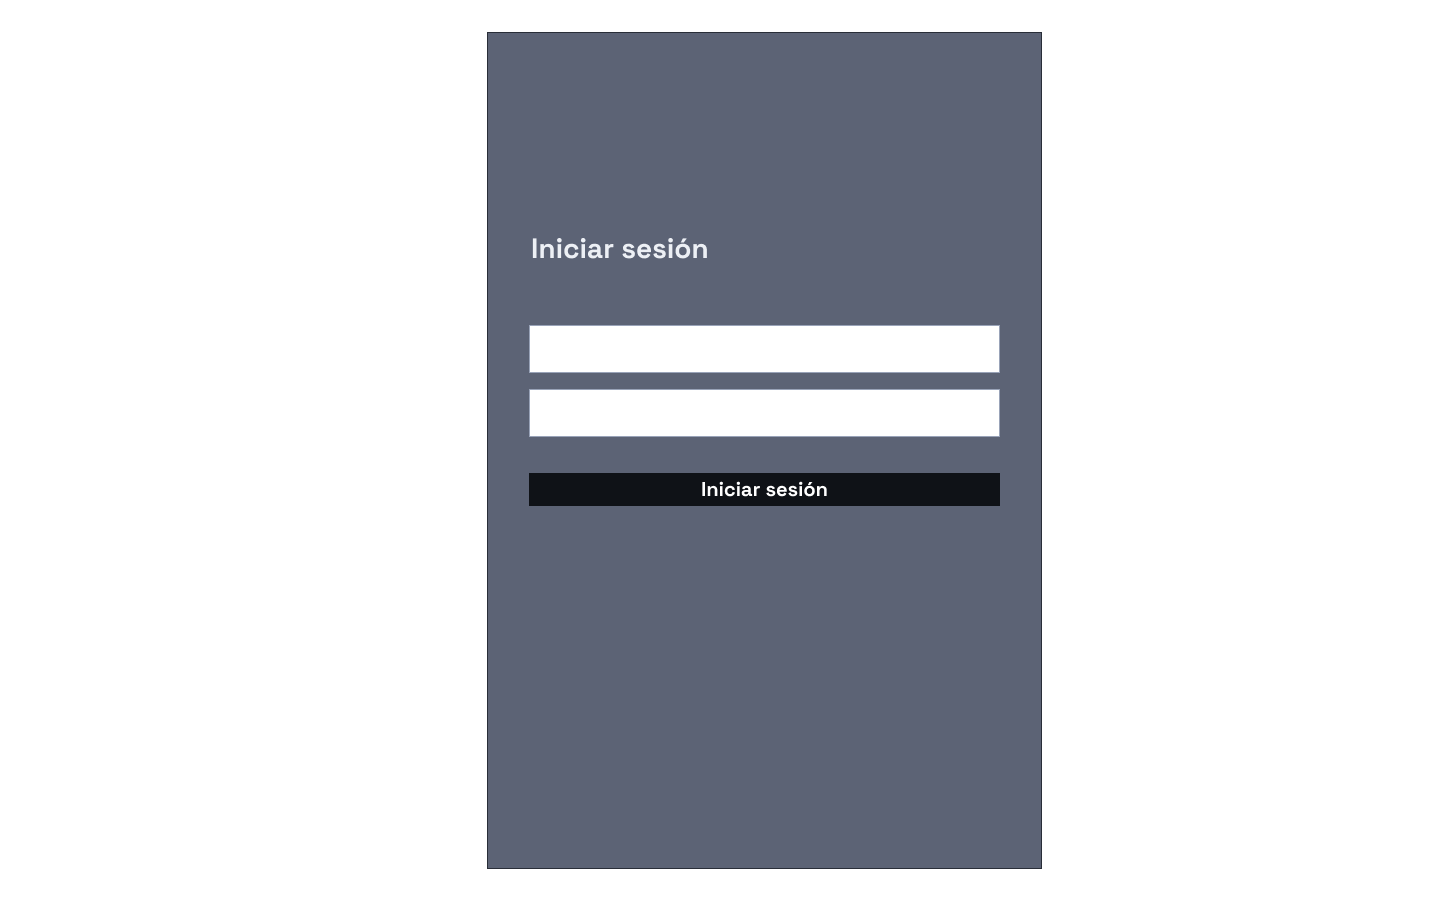
\includegraphics[width=0.5\linewidth]{img/img_2430124/figma/mockups/mockup_login.png}
    \caption{Mockup de la pantalla de inicio de sesión.}
    \label{fig:mockup_login}
\end{figure}

\begin{figure}[!tbh]
    \centering
    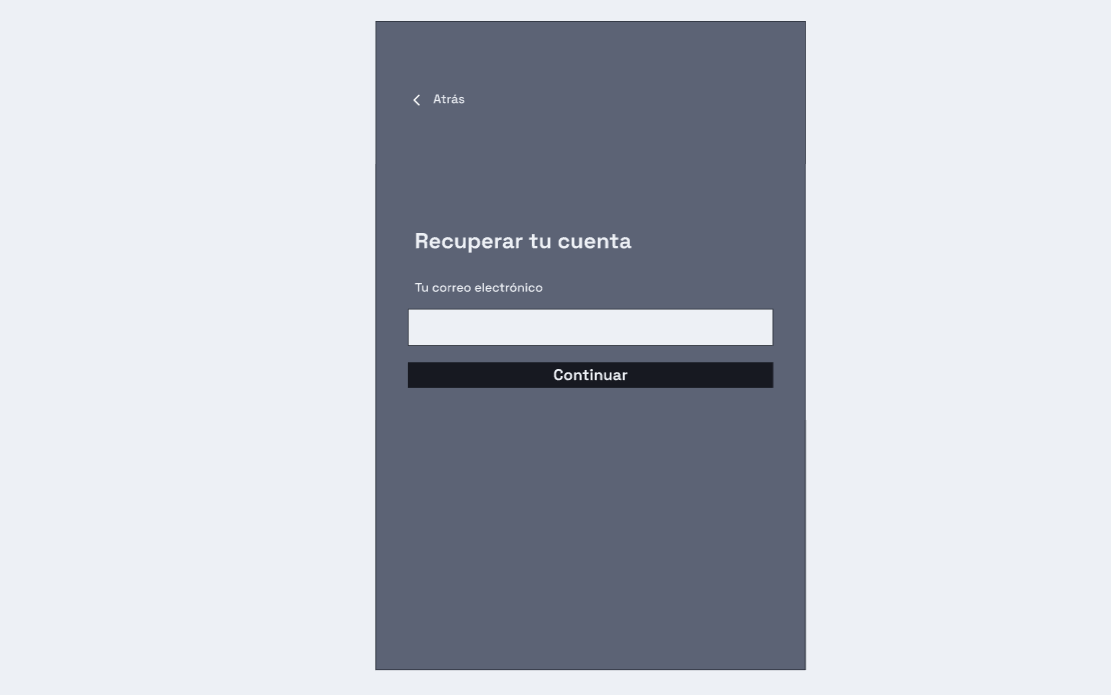
\includegraphics[width=0.5\linewidth]{img/img_2430124/figma/mockups/mockup_recuperar_cuenta.png}
    \caption{Mockup para recuperar cuenta.}
    \label{fig:mockup_recuperar_cuenta}
\end{figure}

\begin{figure}[!tbh]
    \centering
    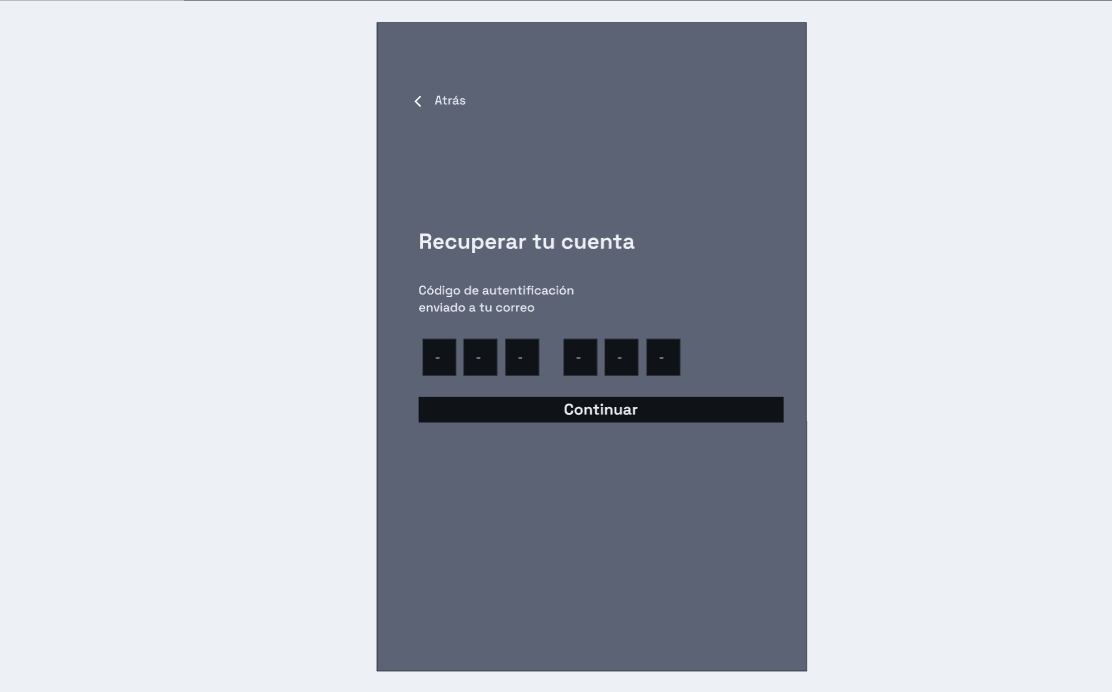
\includegraphics[width=0.5\linewidth]{img/img_2430124/figma/mockups/mockup_codigo_seguridad.png}
    \caption{Mockup para código de seguridad.}
    \label{fig:mockup_codigo_seguridad}
\end{figure}

\begin{figure}[!tbh]
    \centering
    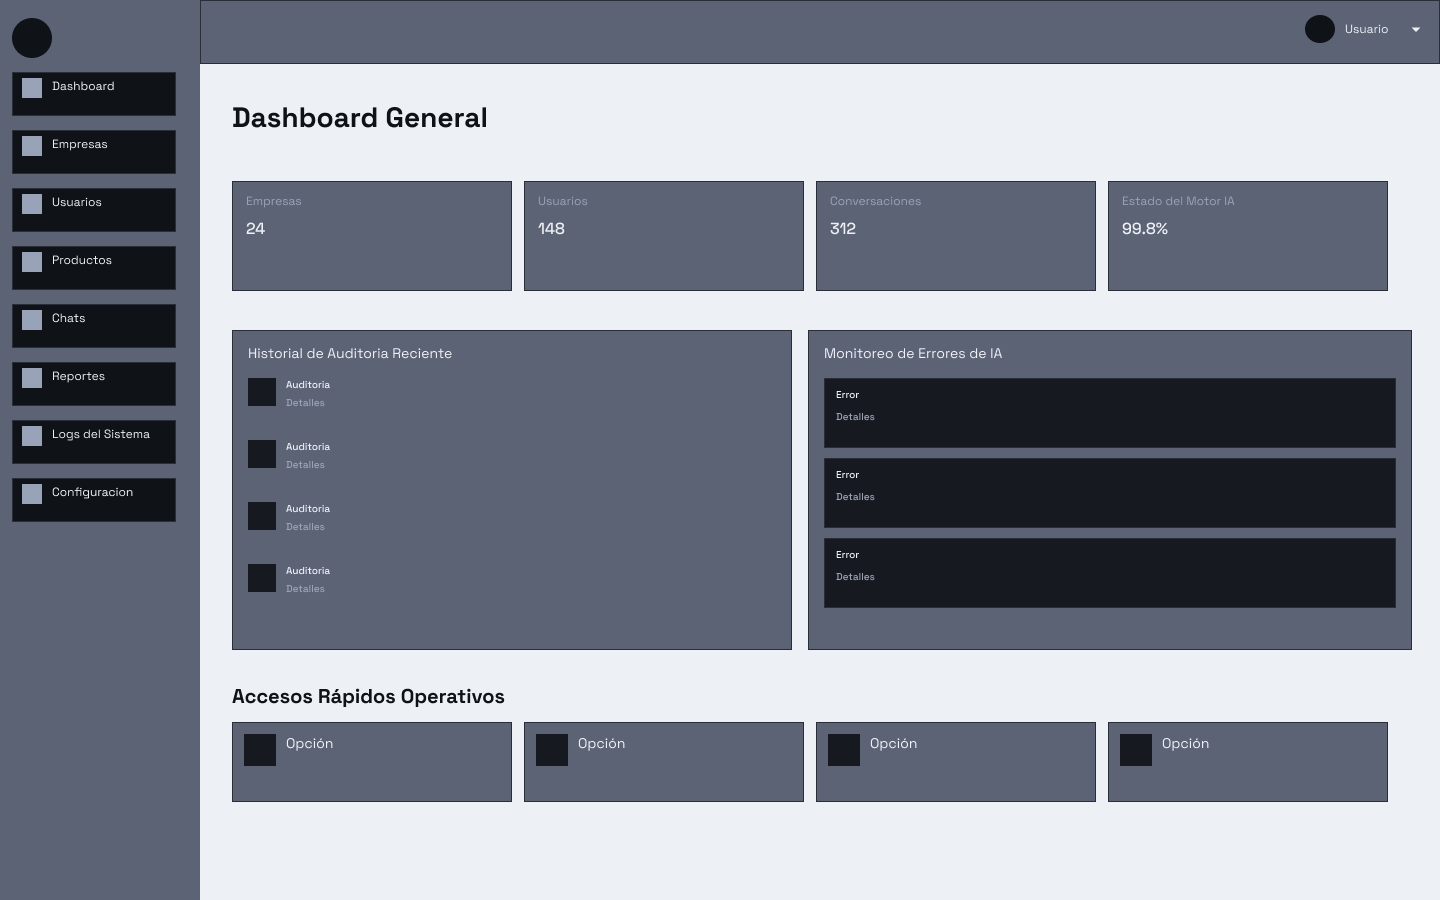
\includegraphics[width=0.5\linewidth]{img/img_2430124/figma/mockups/mockup_admin_dashboard.png}
    \caption{Mockup para el panel de administración.}
    \label{fig:mockup_admin_dashboard}
\end{figure}

\begin{figure}[!tbh]
    \centering
    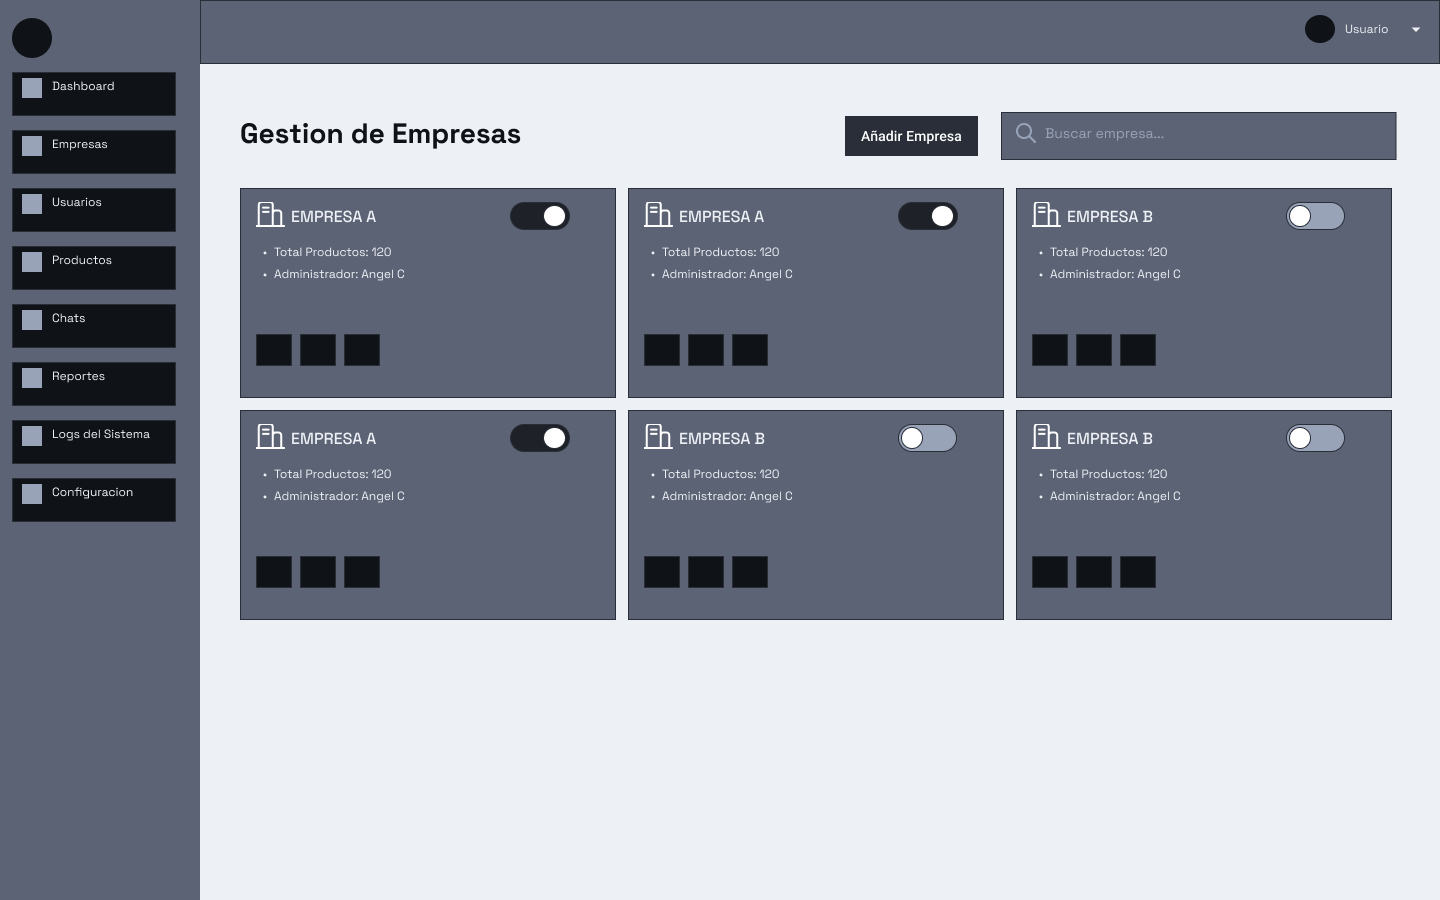
\includegraphics[width=0.5\linewidth]{img/img_2430124/figma/mockups/mockup_empresas.png}
    \caption{Mockup para el apartado de gestión de empresas.}
    \label{fig:mockup_empresas}
\end{figure}

\begin{figure}[!tbh]
    \centering
    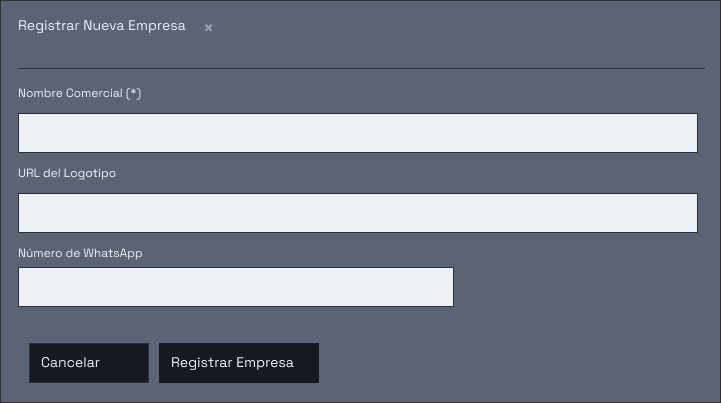
\includegraphics[width=0.5\linewidth]{img/img_2430124/figma/mockups/mockup_modal_nueva_empresa.png}
    \caption{Mockup para el modal de nueva empresa.}
    \label{fig:mockup_modal_nueva_empresa}
\end{figure}

\begin{figure}[!tbh]
    \centering
    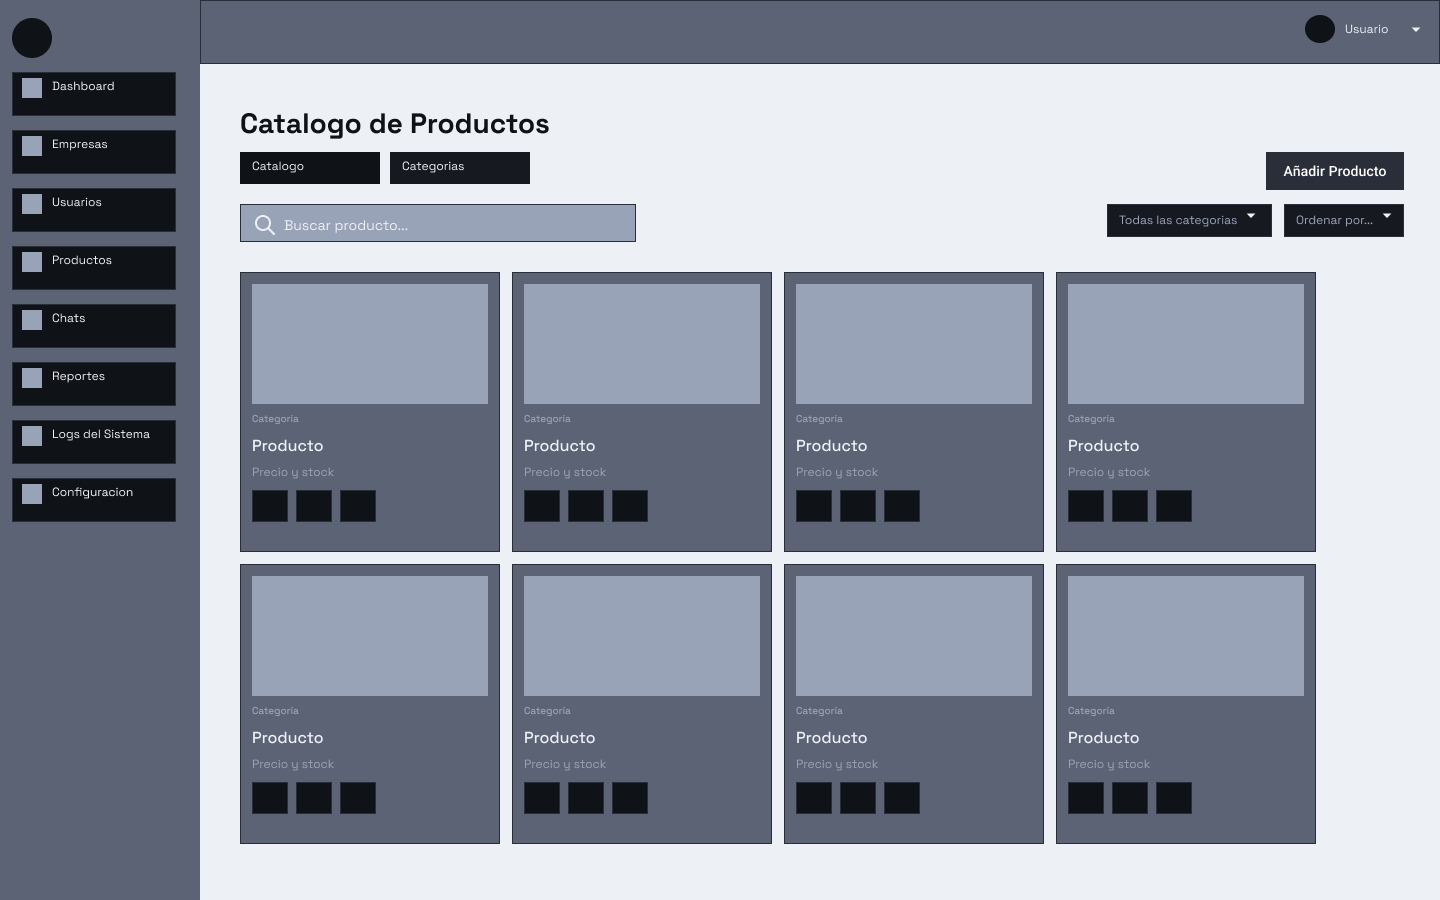
\includegraphics[width=0.5\linewidth]{img/img_2430124/figma/mockups/mockup_productos_catalogo.png}
    \caption{Mockup para el catálogo de productos.}
    \label{fig:mockup_productos_catalogo}
\end{figure}

\begin{figure}[!tbh]
    \centering
    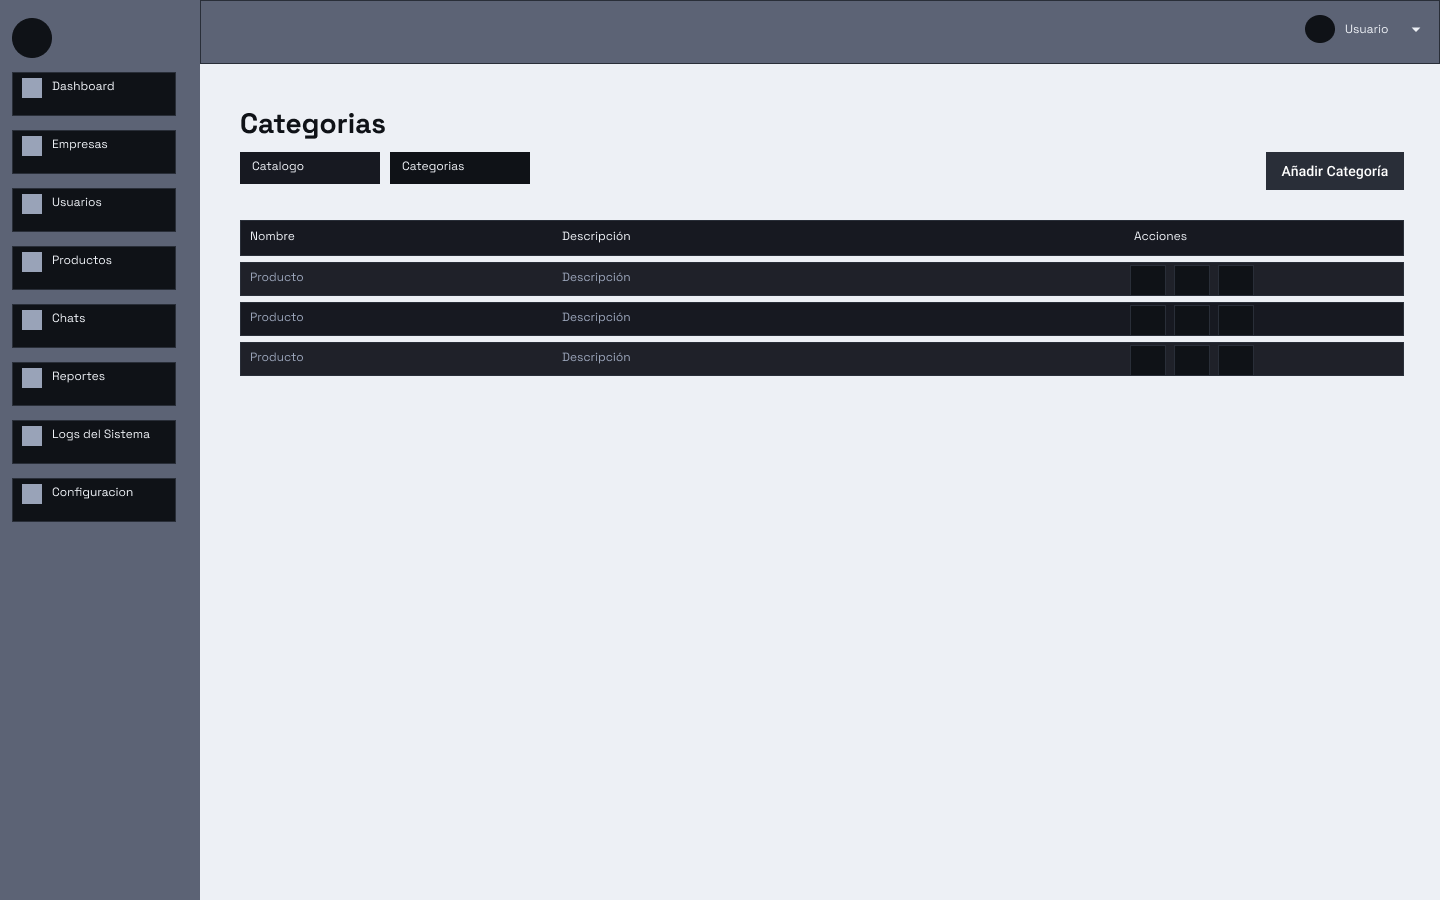
\includegraphics[width=0.5\linewidth]{img/img_2430124/figma/mockups/mockup_productos_categorias.png}
    \caption{Mockup para las categorías de productos.}
    \label{fig:mockup_productos_categorias}
\end{figure}

\begin{figure}[!tbh]
    \centering
    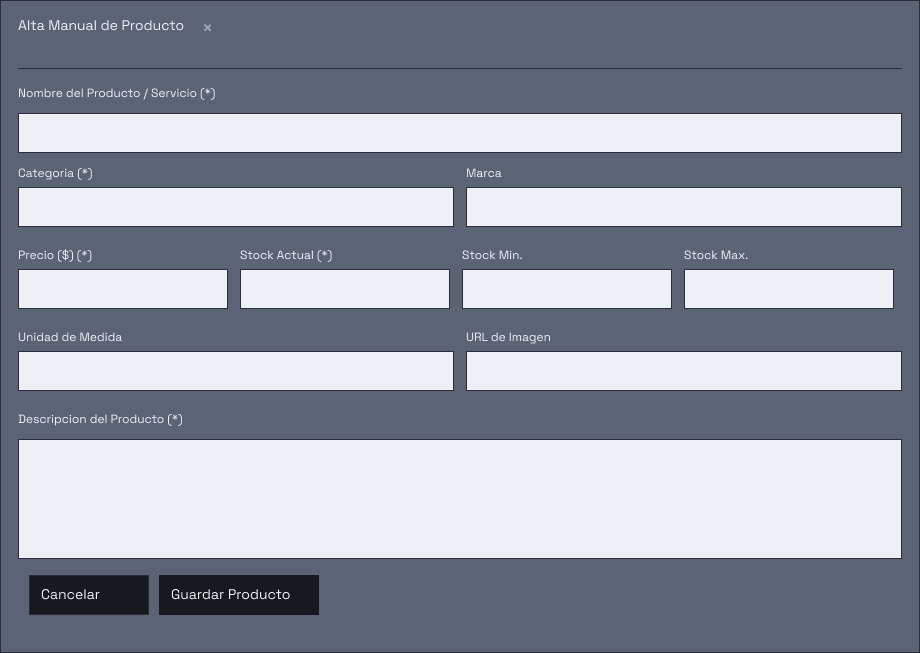
\includegraphics[width=0.5\linewidth]{img/img_2430124/figma/mockups/mockup_modal_alta_manual_producto.png}
    \caption{Mockup para el modal de alta manual de producto.}
    \label{fig:mockup_modal_alta_manual_producto}
\end{figure}

\begin{figure}[!tbh]
    \centering
    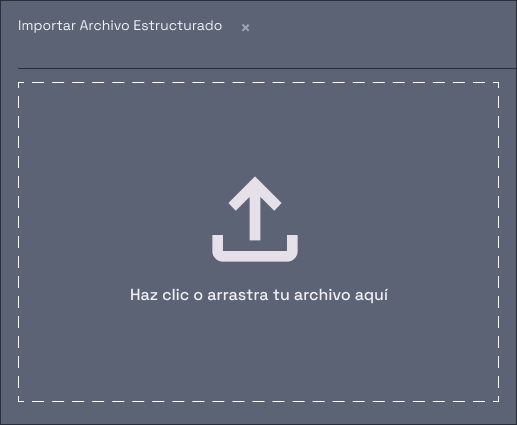
\includegraphics[width=0.5\linewidth]{img/img_2430124/figma/mockups/mockup_modal_importar_por_csv.png}
    \caption{Mockup para el modal de importación de productos por CSV.}
    \label{fig:mockup_modal_importar_por_csv}
\end{figure}

\begin{figure}[!tbh]
    \centering
    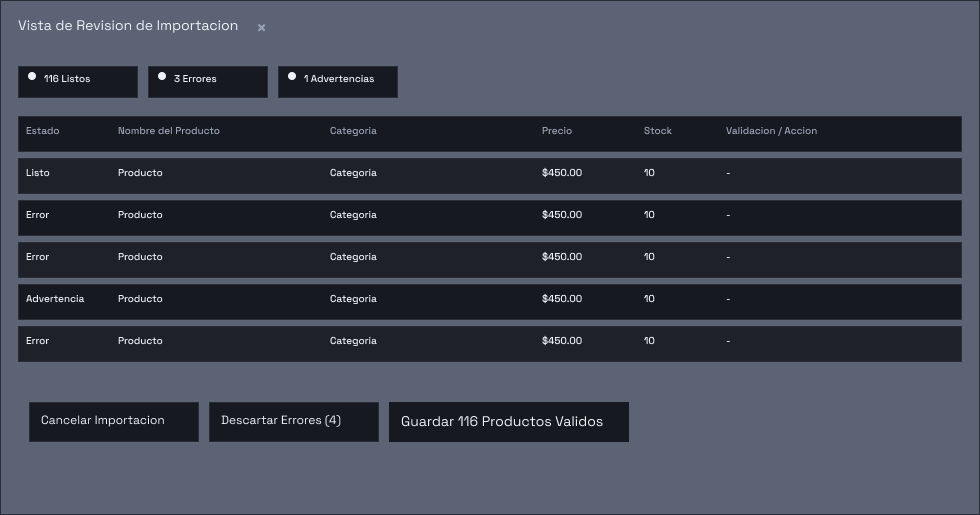
\includegraphics[width=0.5\linewidth]{img/img_2430124/figma/mockups/mockup_modal_revision_importacion.png}
    \caption{Mockup para el modal de revisión de importación de productos.}
    \label{fig:mockup_modal_revision_importacion}
\end{figure}

\begin{figure}[!tbh]
    \centering
    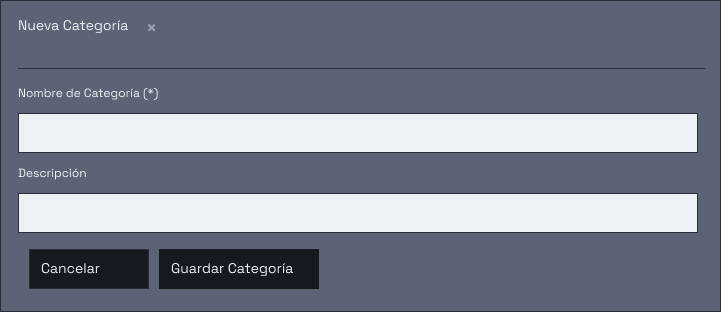
\includegraphics[width=0.5\linewidth]{img/img_2430124/figma/mockups/mockup_modal_nueva_categoria.png}
    \caption{Mockup para el modal de nueva categoría.}
    \label{fig:mockup_modal_nueva_categoria}
\end{figure}

\begin{figure}[!tbh]
    \centering
    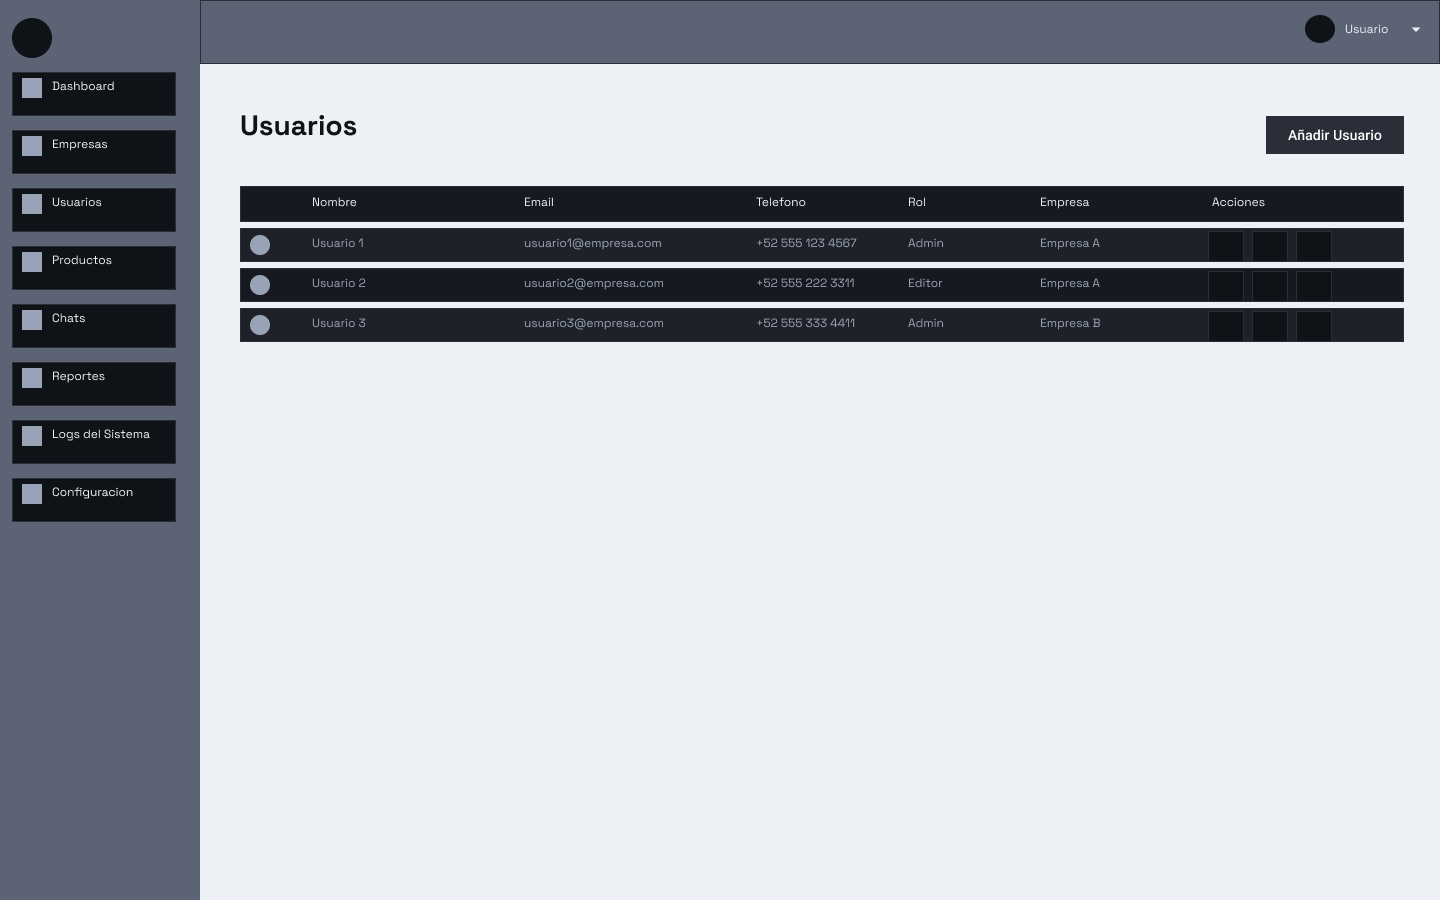
\includegraphics[width=0.5\linewidth]{img/img_2430124/figma/mockups/mockup_usuarios.png}
    \caption{Mockup para el panel de usuarios.}
    \label{fig:mockup_usuarios}
\end{figure}

\begin{figure}[!tbh]
    \centering
    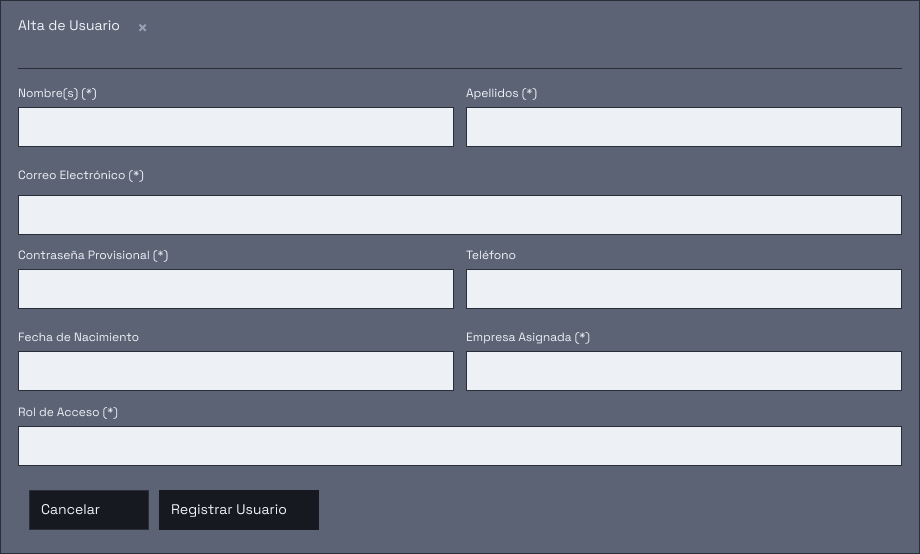
\includegraphics[width=0.5\linewidth]{img/img_2430124/figma/mockups/mockup_modal_nuevo_usuario.png}
    \caption{Mockup para el modal de nuevo usuario.}
    \label{fig:mockup_modal_nuevo_usuario}
\end{figure}

\begin{figure}[!tbh]
    \centering
    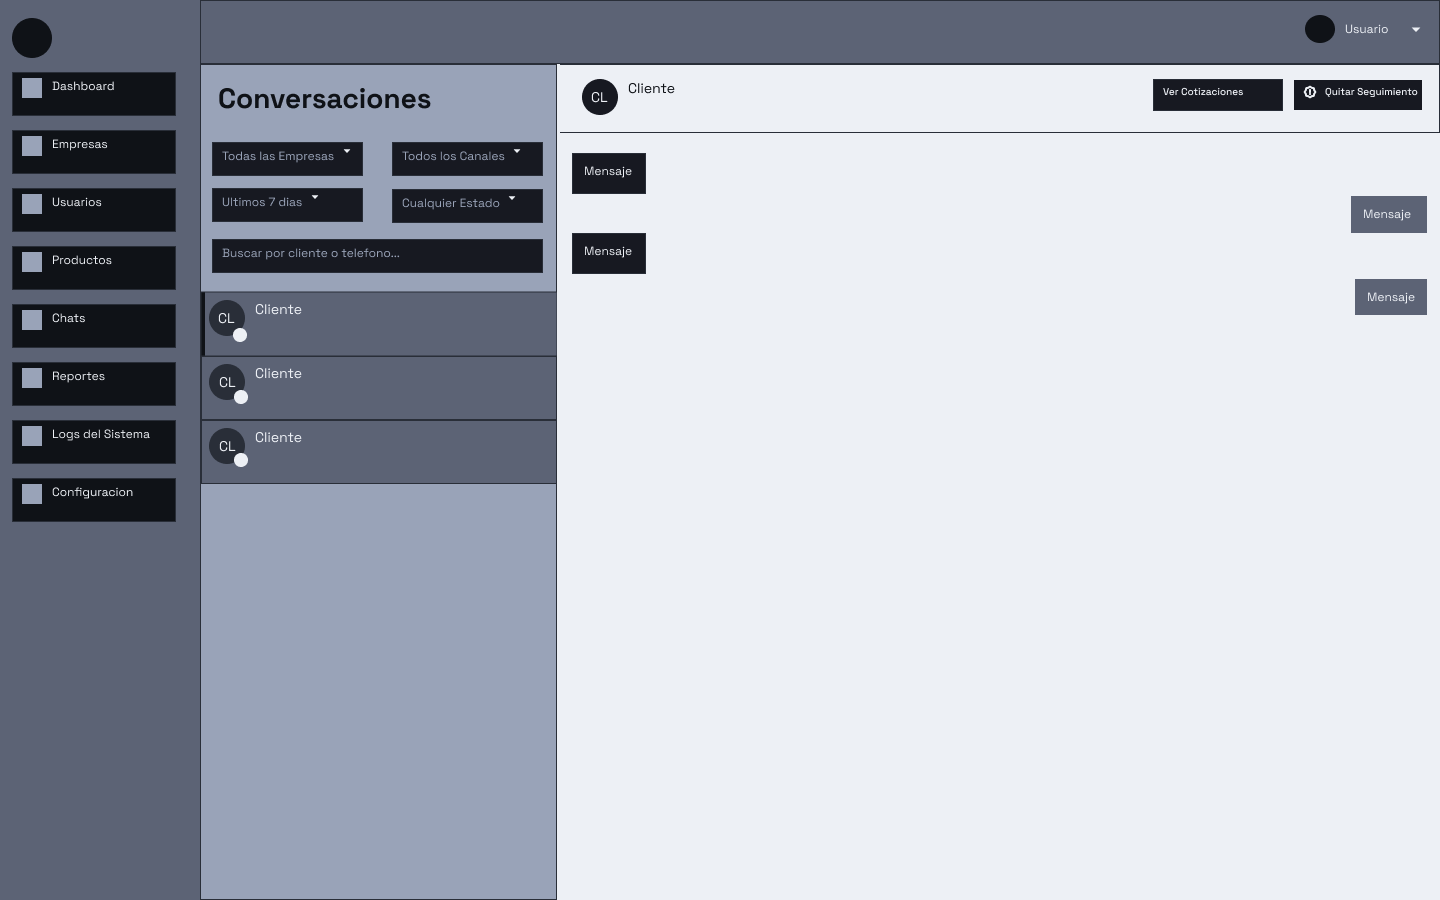
\includegraphics[width=0.5\linewidth]{img/img_2430124/figma/mockups/mockup_chats_historial.png}
    \caption{Mockup para el historial de chats.}
    \label{fig:mockup_chats_historial}
\end{figure}

\begin{figure}[!tbh]
    \centering
    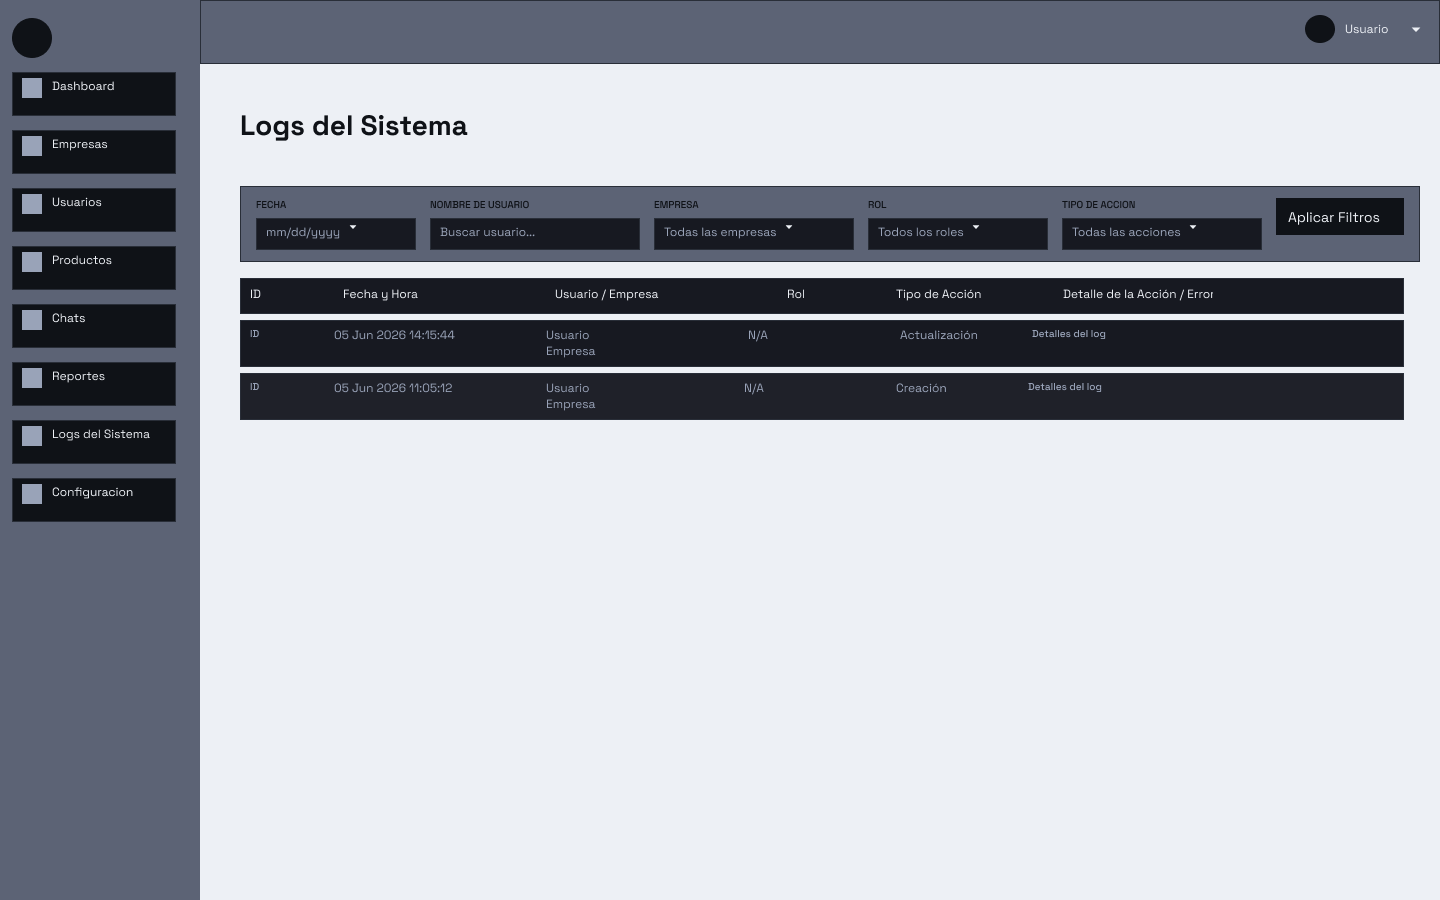
\includegraphics[width=0.5\linewidth]{img/img_2430124/figma/mockups/mockup_logs.png}
    \caption{Mockup para el panel de logs.}
    \label{fig:mockup_logs}
\end{figure}

\begin{figure}[!tbh]
    \centering
    
\includegraphics[width=0.5\linewidth]{img/img_2430124/figma/mockups/mockup_widget.png}
    \caption{Mockup para el widget web de chat.}
    \label{fig:mockup_widget}
\end{figure}

\begin{figure}[!tbh]
    \centering
    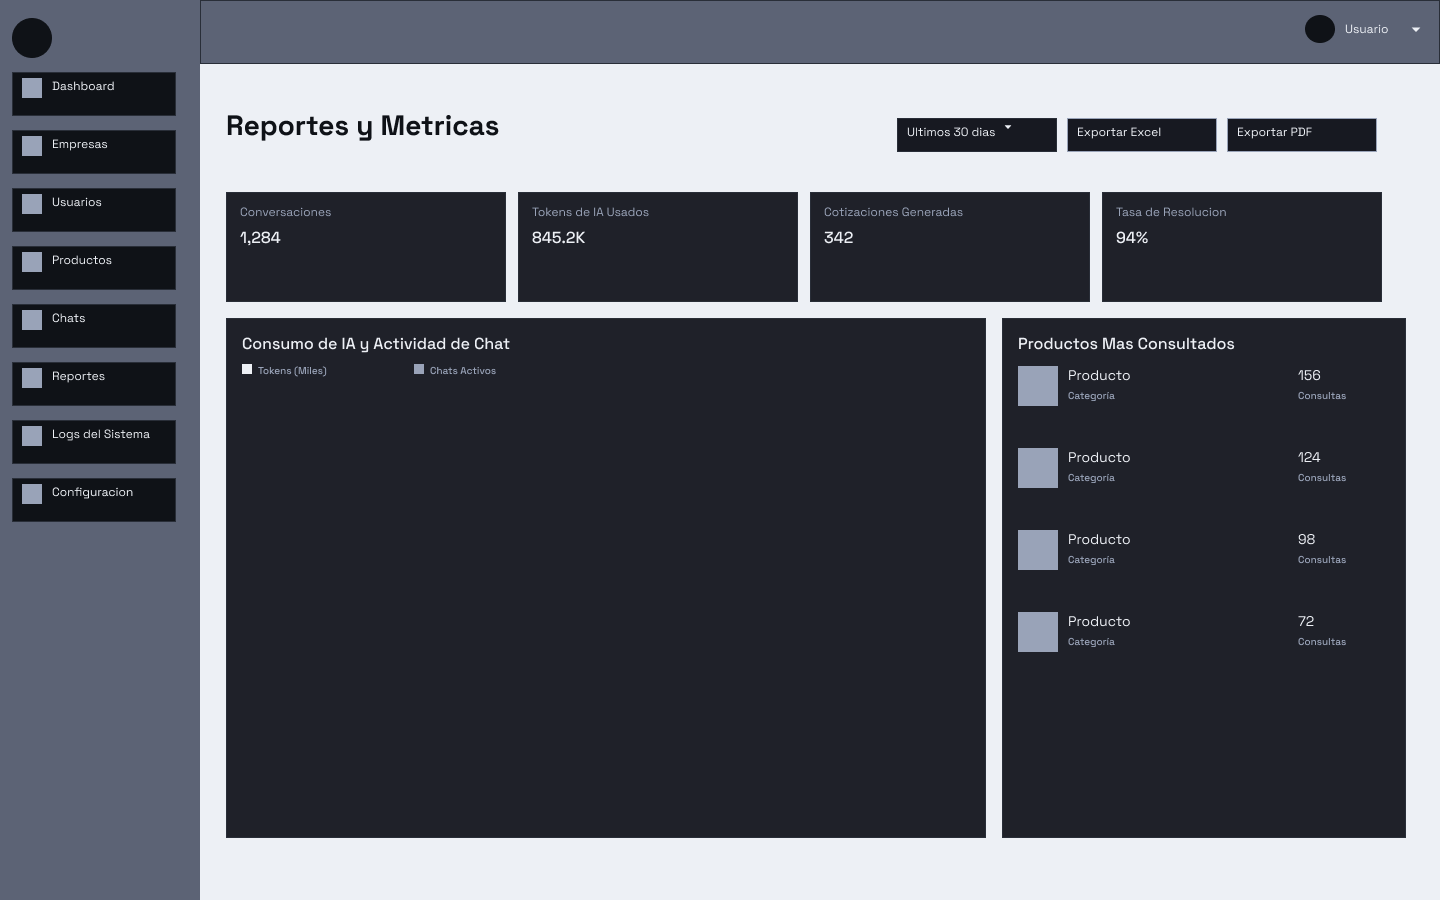
\includegraphics[width=0.5\linewidth]{img/img_2430124/figma/mockups/mockup_reportes.png}
    \caption{Mockup para el panel de reportes.}
    \label{fig:mockup_reportes}
\end{figure}

\begin{figure}[!tbh]
    \centering
    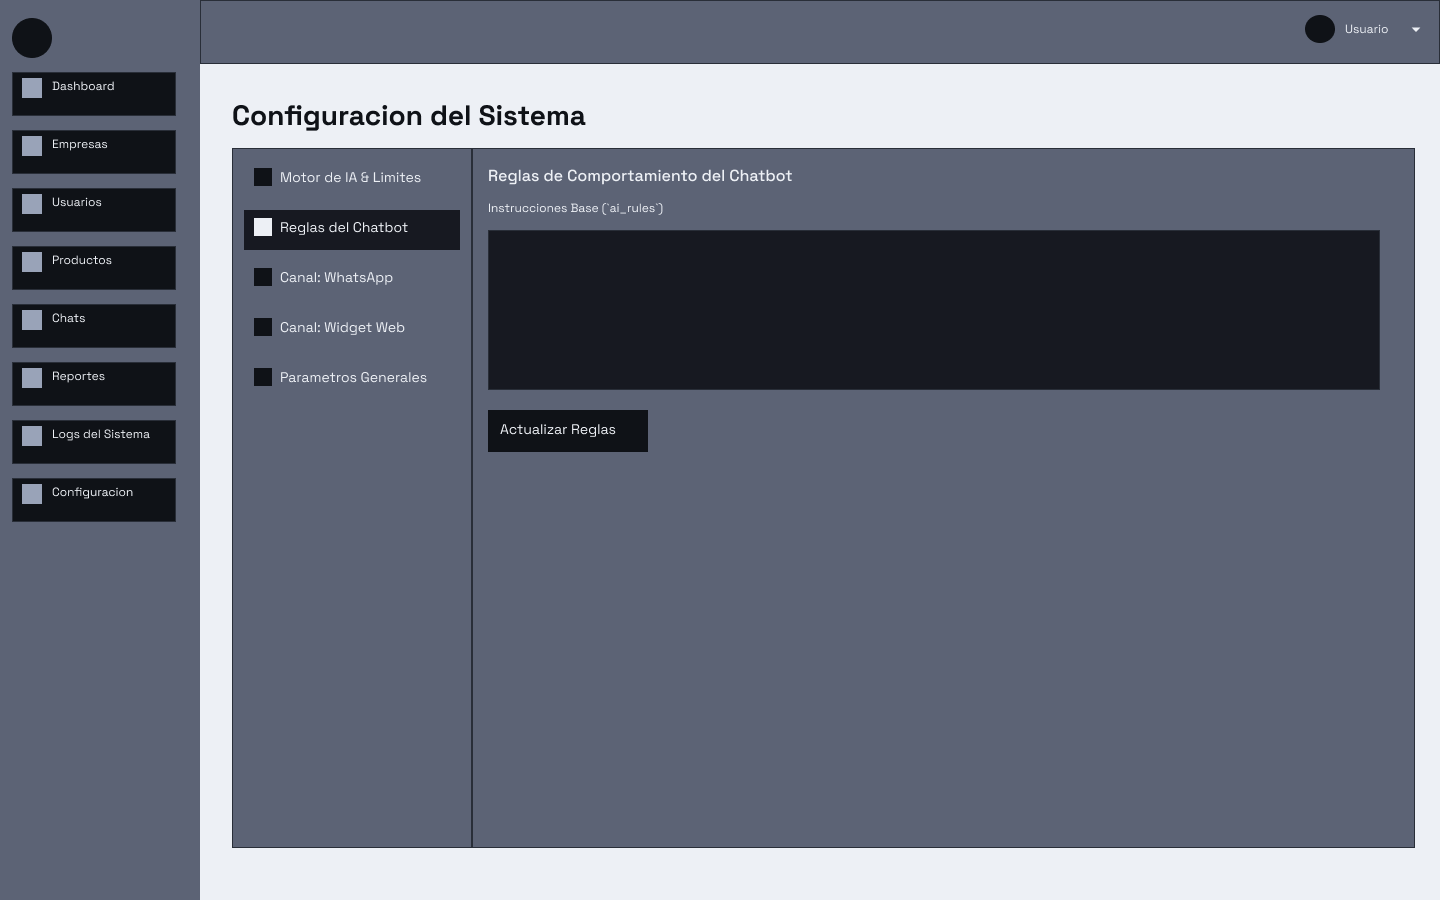
\includegraphics[width=0.5\linewidth]{img/img_2430124/figma/mockups/mockup_reglas.png}
    \caption{Mockup para el panel de configuración de reglas del modelo de IA.}
    \label{fig:mockup_reglas}
\end{figure}

\begin{figure}[!tbh]
    \centering
    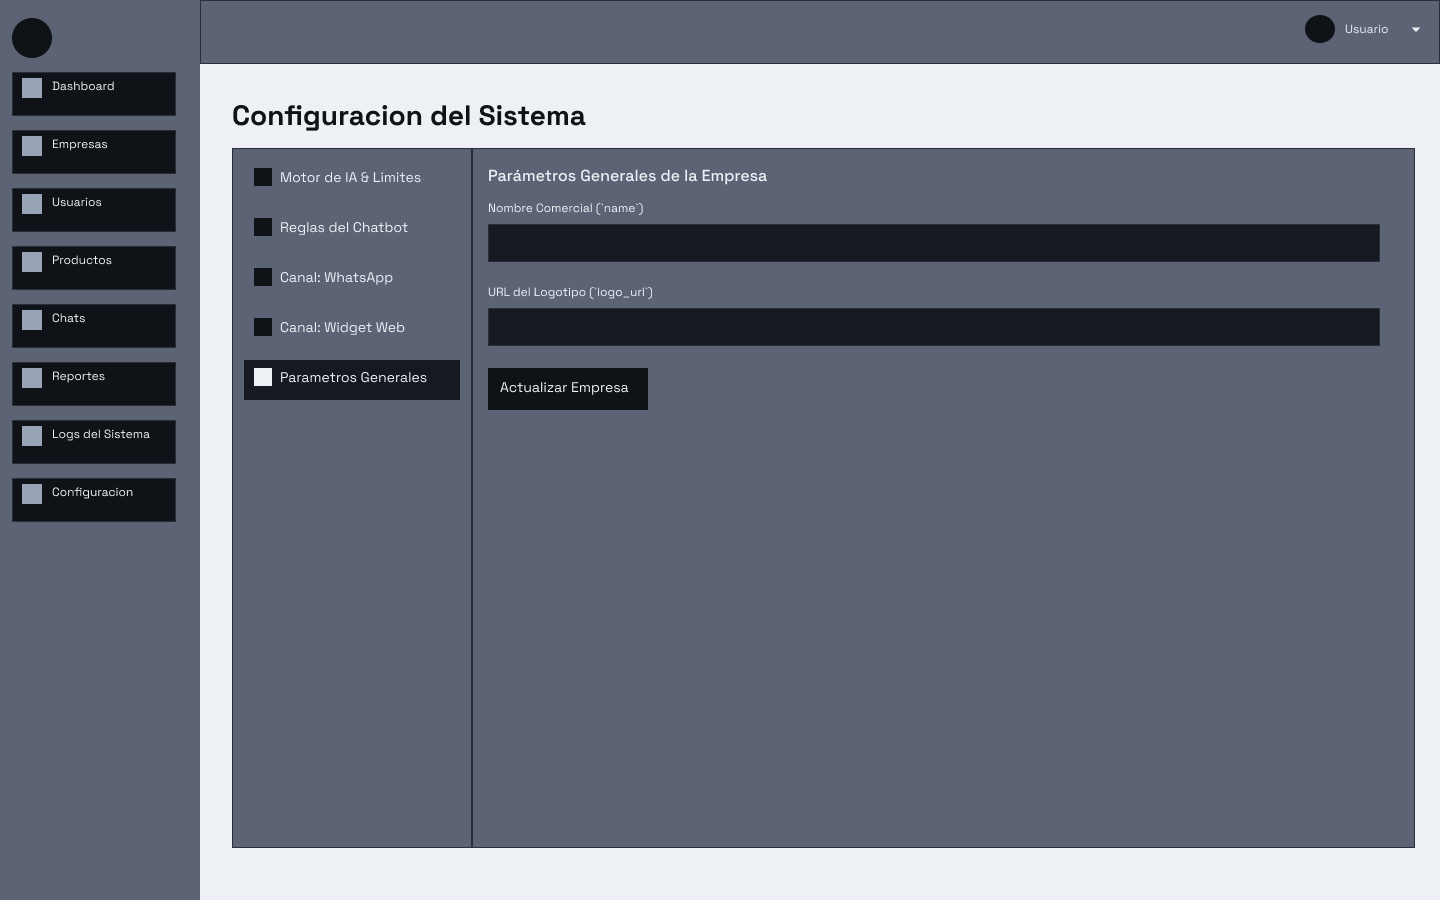
\includegraphics[width=0.5\linewidth]{img/img_2430124/figma/mockups/mockup_parametros.png}
    \caption{Mockup para el panel de configuración de parámetros del modelo de IA.}
    \label{fig:mockup_parametros}
\end{figure}

\begin{figure}[!tbh]
    \centering
    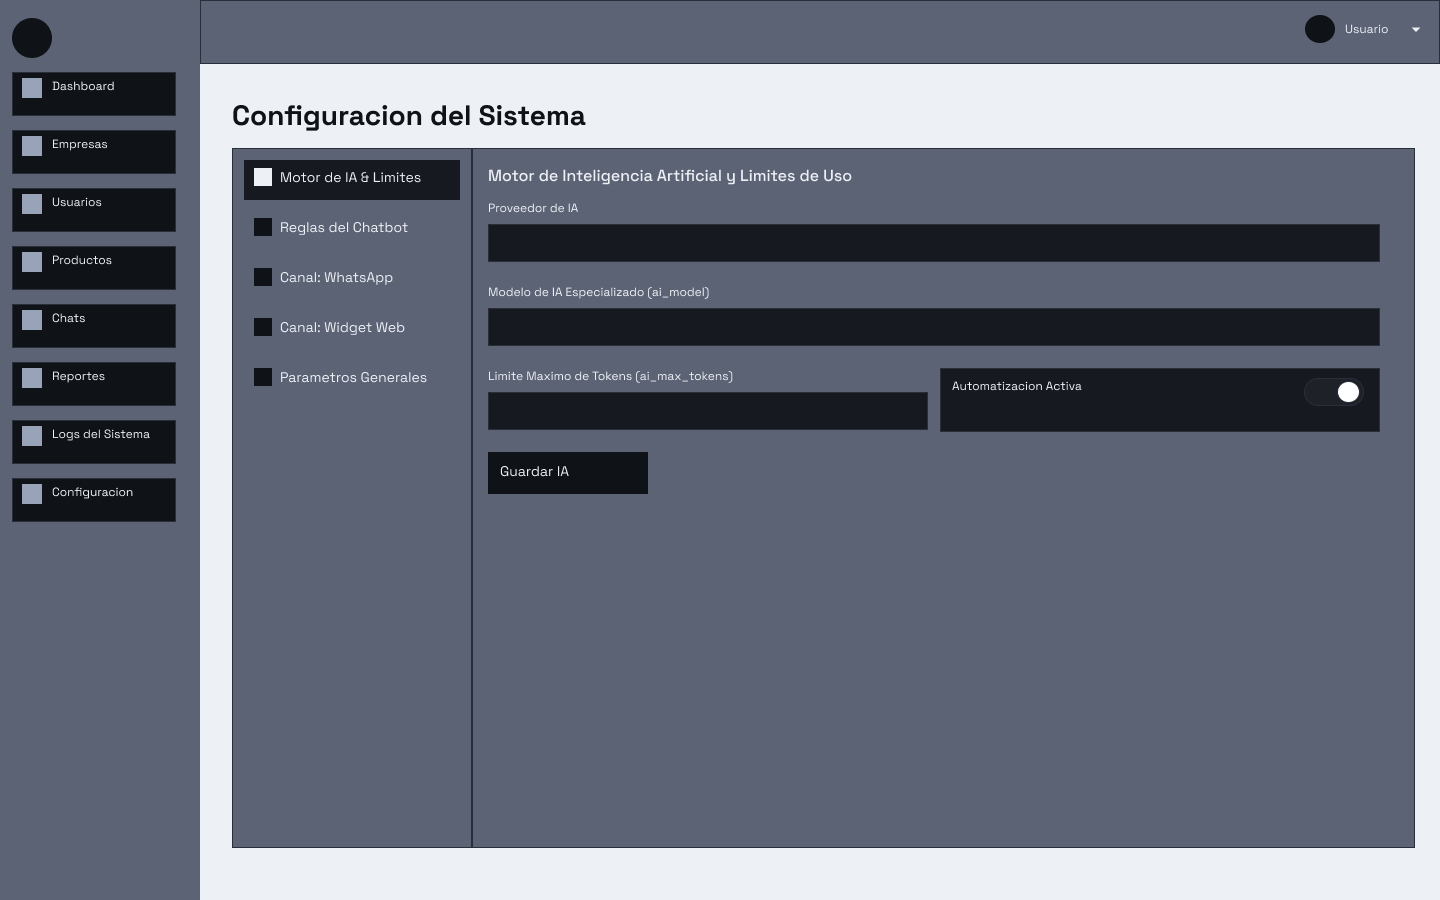
\includegraphics[width=0.5\linewidth]{img/img_2430124/figma/mockups/mockup_motor_ia.png}
    \caption{Mockup para el panel de configuración del motor de IA.}
    \label{fig:mockup_motor_ia}
\end{figure}

\begin{figure}[!tbh]
    \centering
    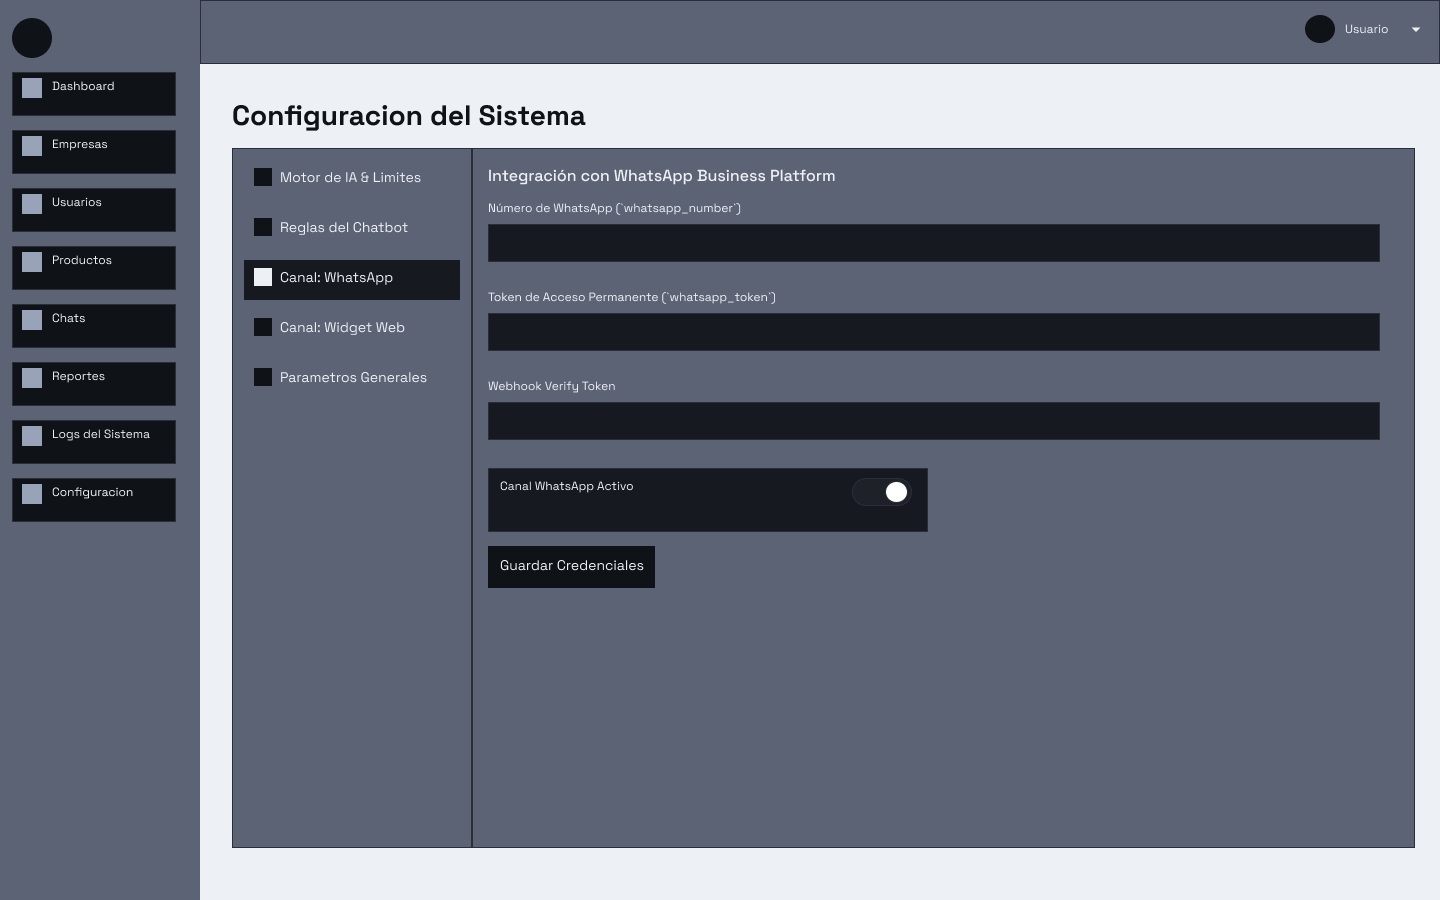
\includegraphics[width=0.5\linewidth]{img/img_2430124/figma/mockups/mockup_canal_whatsapp.png}
    \caption{Mockup para el panel de configuración del canal de WhatsApp.}
    \label{fig:mockup_canal_whatsapp}
\end{figure}

\begin{figure}[!tbh]
    \centering
    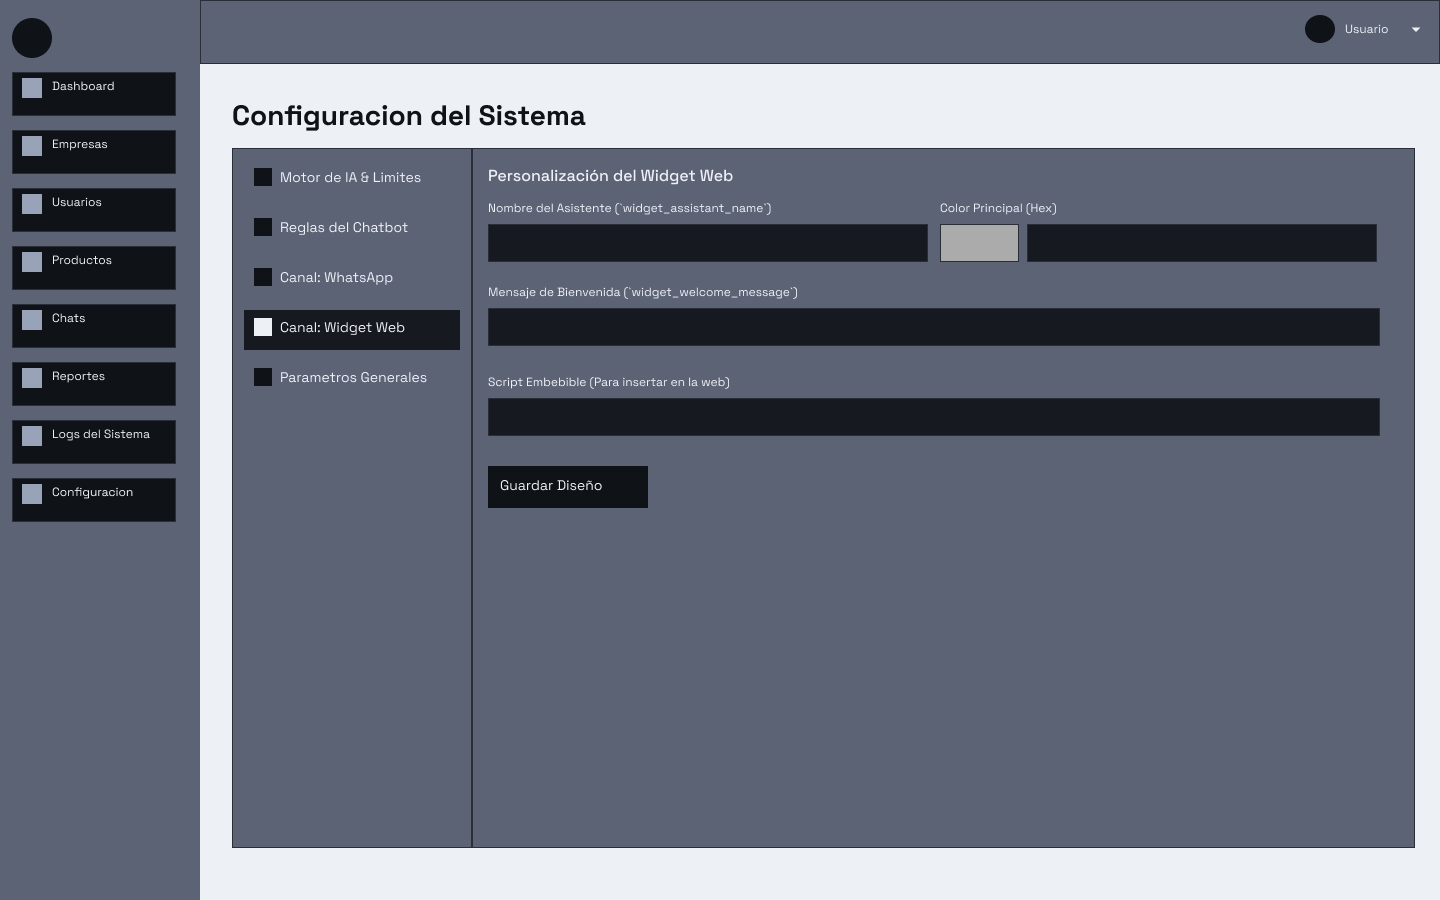
\includegraphics[width=0.5\linewidth]{img/img_2430124/figma/mockups/mockup_canal_widget.png}
    \caption{Mockup para el panel de configuración del canal de widget.}
    \label{fig:mockup_canal_widget}
\end{figure}

\subsection{Diseño UX}
\label{sec:diseno_ux}

\begin{figure}[!tbh]
    \centering
    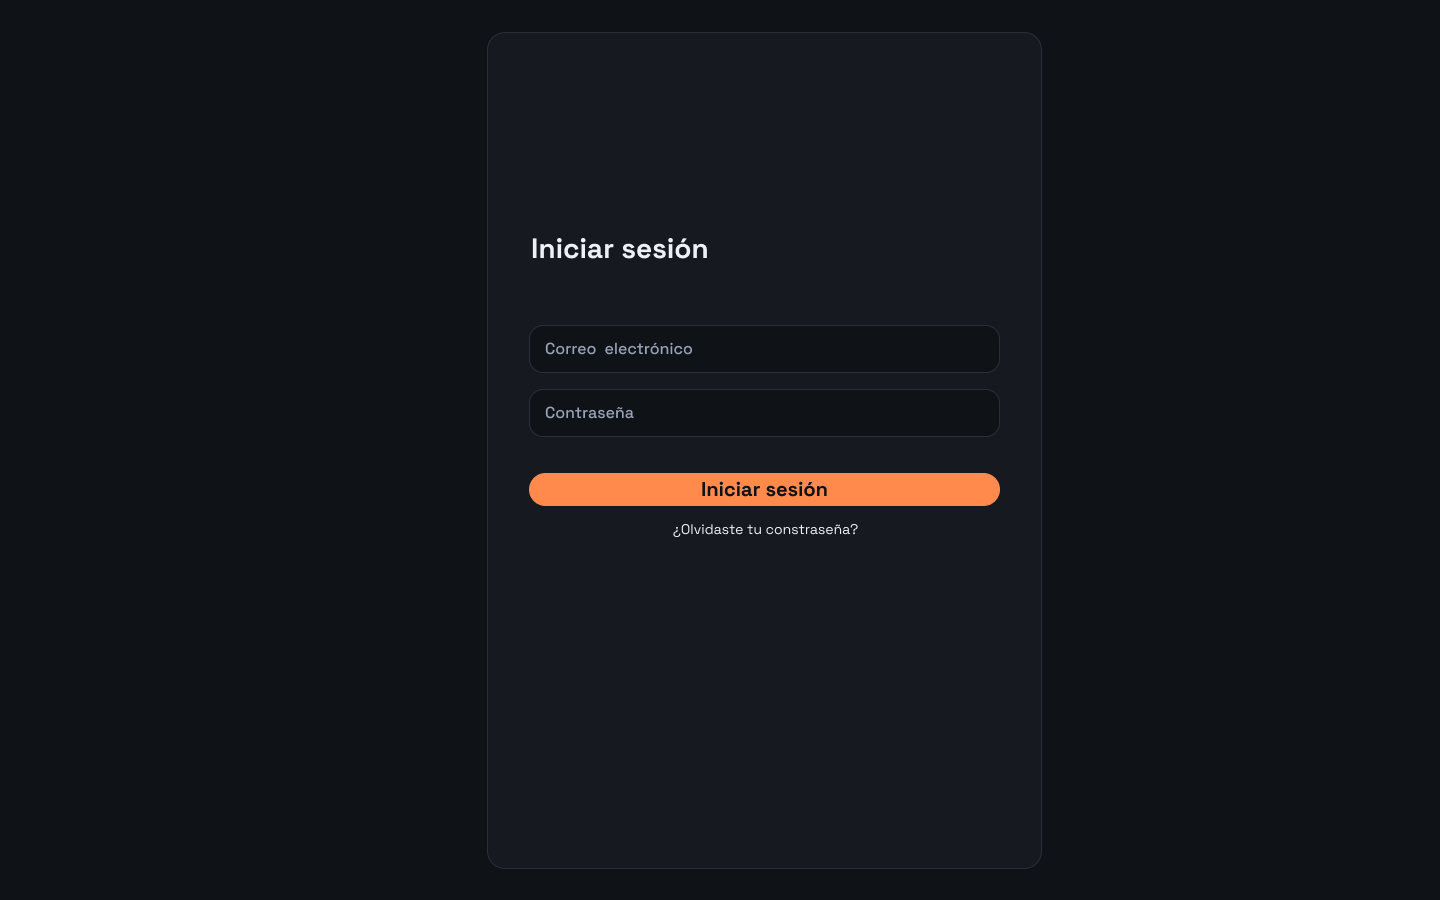
\includegraphics[width=0.5\linewidth]{img/img_2430124/figma/ux/ux_login.png}
    \caption{Diseño UX de la pantalla de inicio de sesión.}
    \label{fig:ux_login}
\end{figure}

\begin{figure}[!tbh]
    \centering
    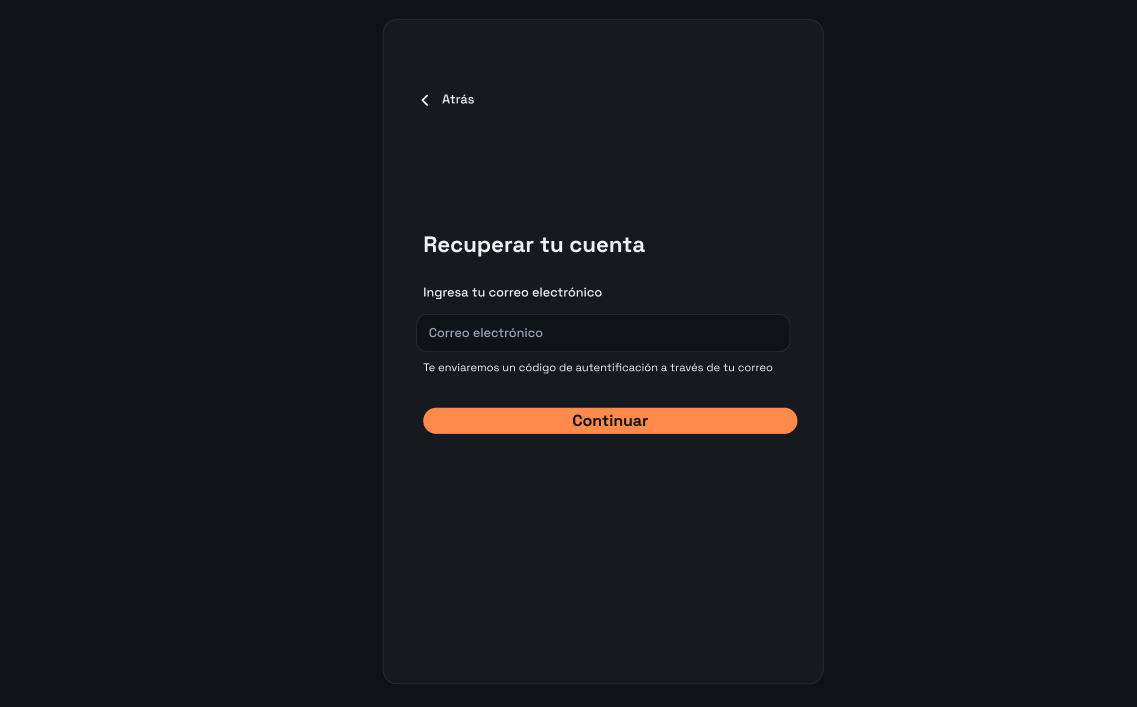
\includegraphics[width=0.5\linewidth]{img/img_2430124/figma/ux/ux_recuperar_cuenta.png}
    \caption{Diseño UX para recuperar cuenta.}
    \label{fig:ux_recuperar_cuenta}
\end{figure}

\begin{figure}[!tbh]
    \centering
    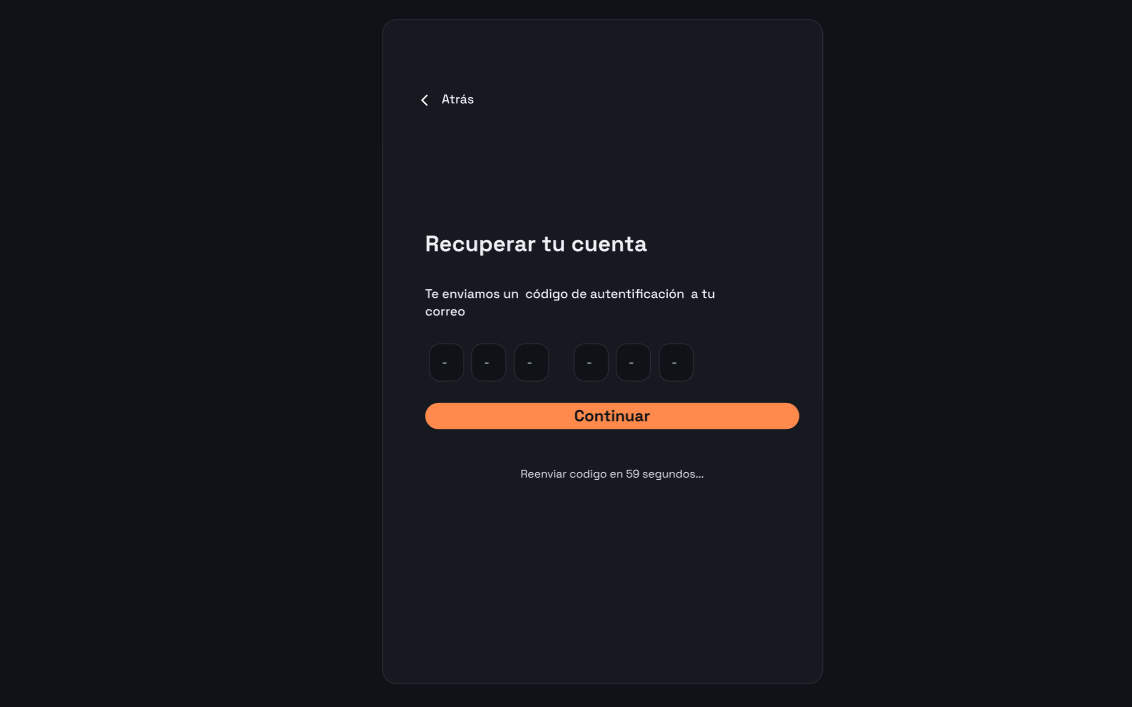
\includegraphics[width=0.5\linewidth]{img/img_2430124/figma/ux/ux_codigo_seguridad.png}
    \caption{Diseño UX para código de seguridad.}
    \label{fig:ux_codigo_seguridad}
\end{figure}

\begin{figure}[!tbh]
    \centering
    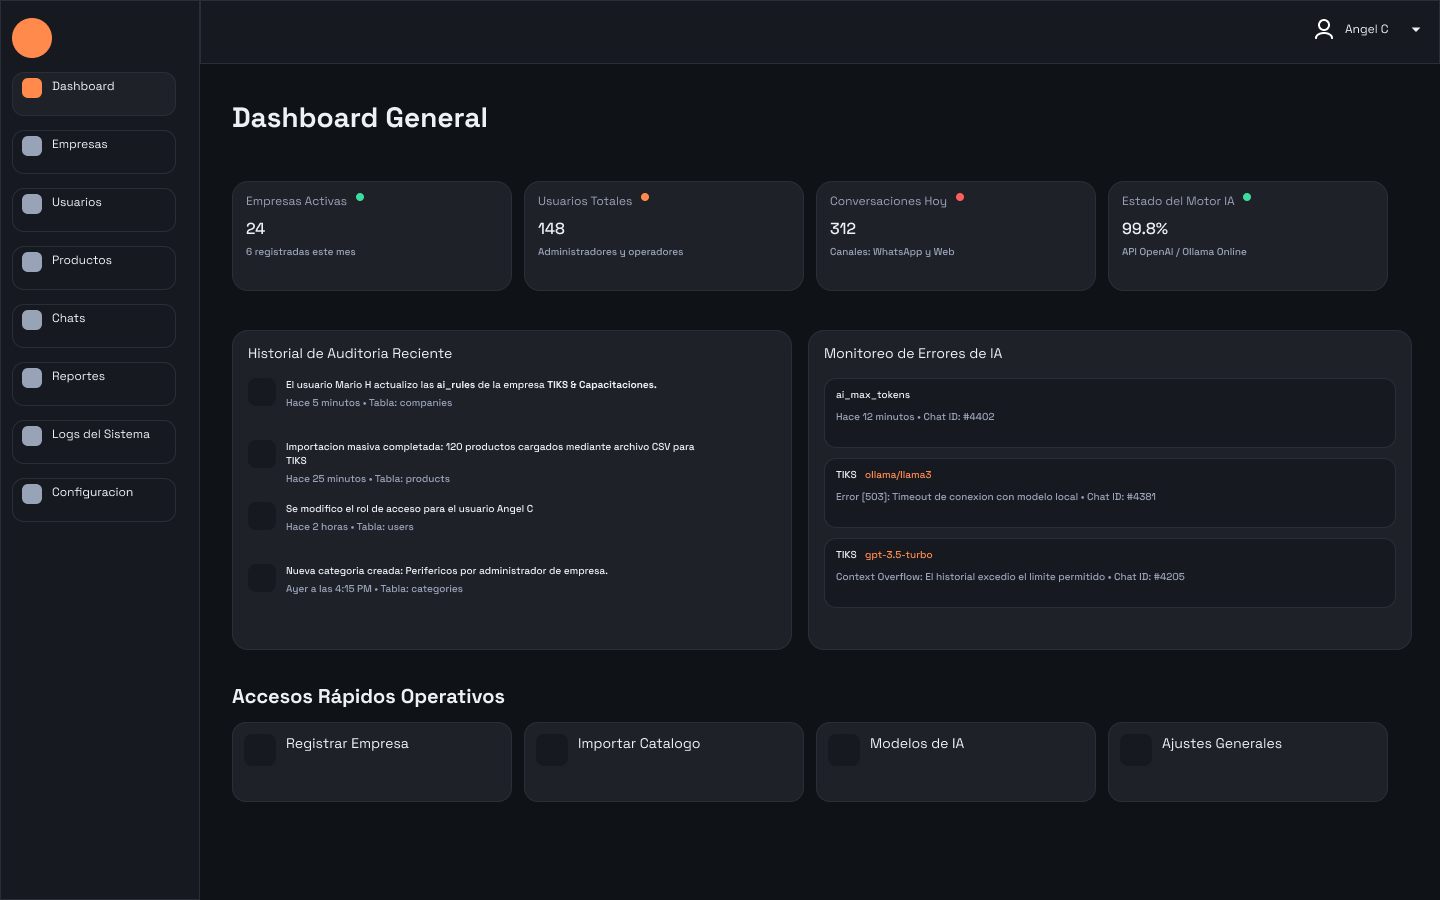
\includegraphics[width=0.5\linewidth]{img/img_2430124/figma/ux/ux_admin_dashboard.png}
    \caption{Diseño UX para el panel de administración.}
    \label{fig:ux_admin_dashboard}
\end{figure}

\begin{figure}[!tbh]
    \centering
    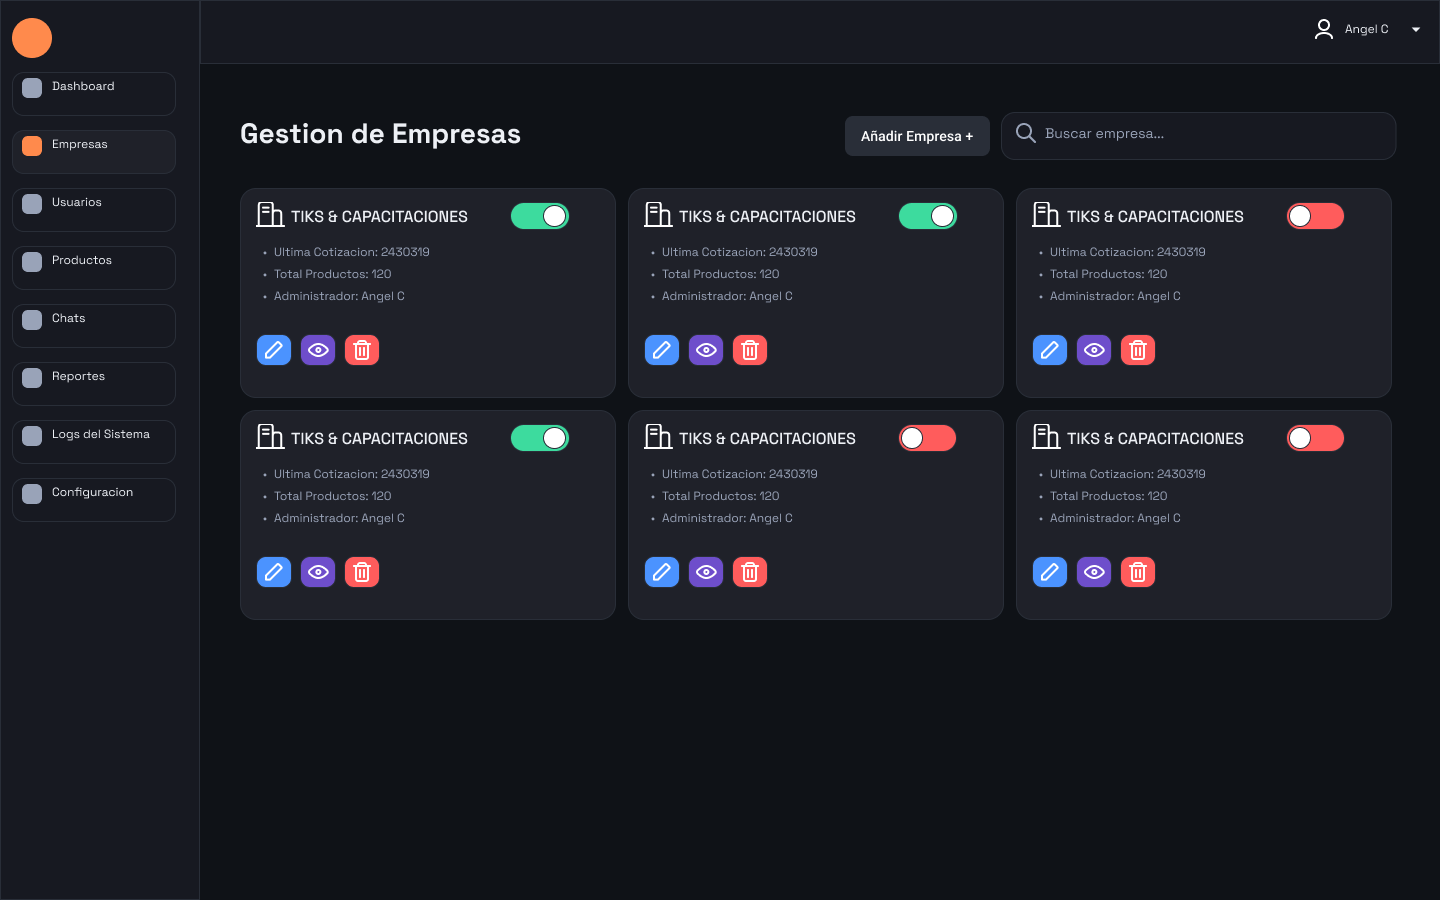
\includegraphics[width=0.5\linewidth]{img/img_2430124/figma/ux/ux_empresas.png}
    \caption{Diseño UX para el apartado de gestión de empresas.}
    \label{fig:ux_empresas}
\end{figure}

\begin{figure}[!tbh]
    \centering
    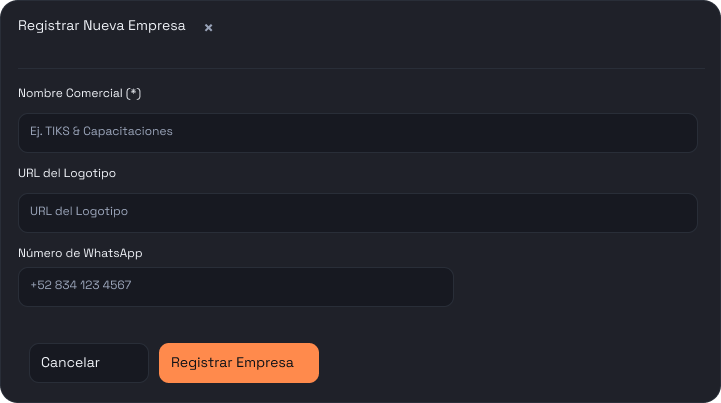
\includegraphics[width=0.5\linewidth]{img/img_2430124/figma/ux/ux_modal_nueva_empresa.png}
    \caption{Diseño UX para el modal de nueva empresa.}
    \label{fig:ux_modal_nueva_empresa}
\end{figure}

\begin{figure}[!tbh]
    \centering
    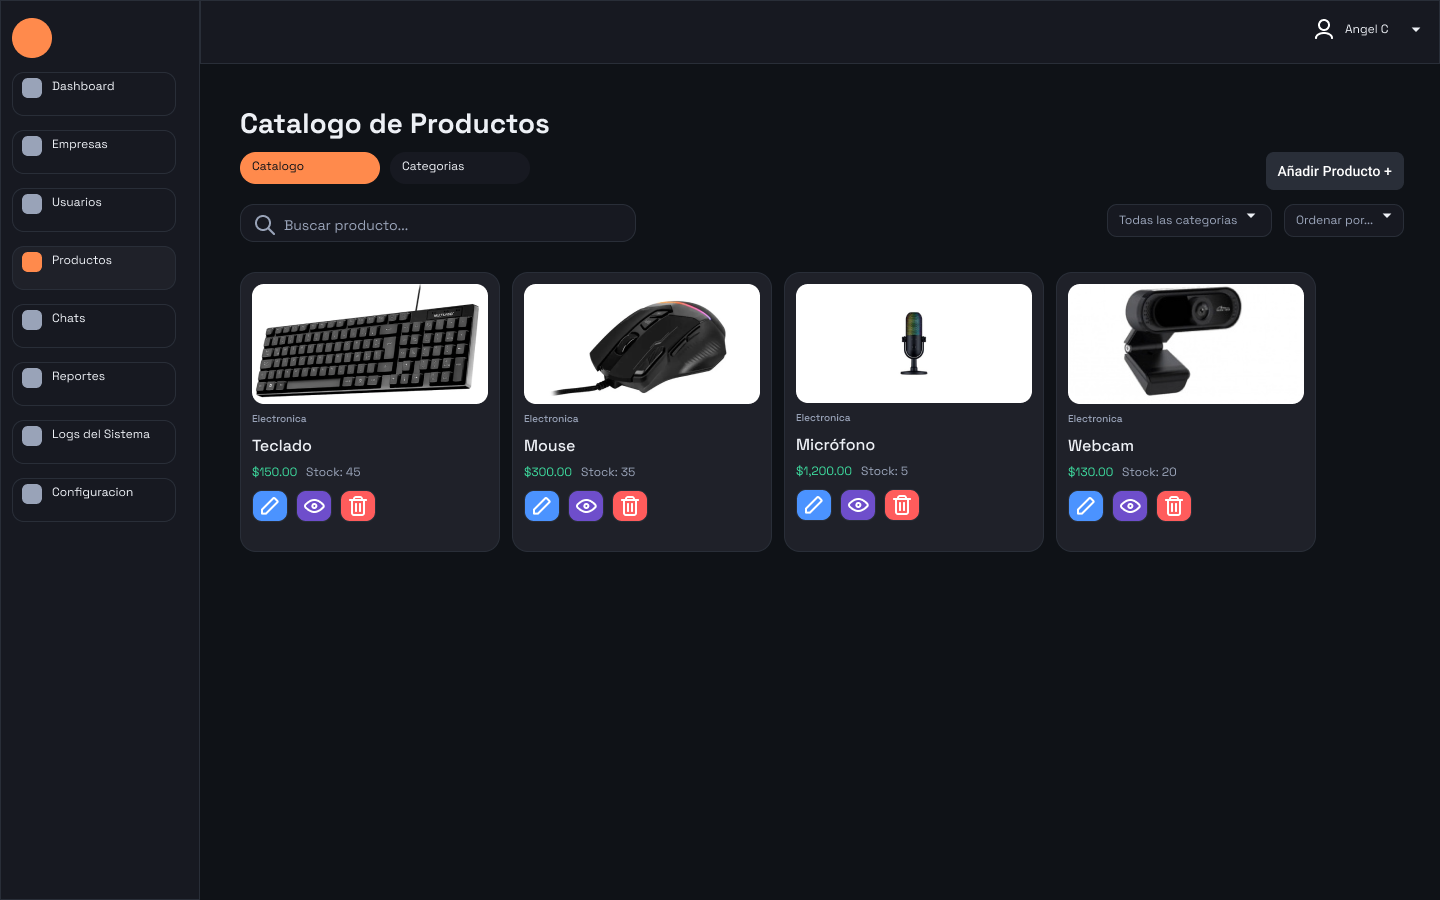
\includegraphics[width=0.5\linewidth]{img/img_2430124/figma/ux/ux_productos_catalogo.png}
    \caption{Diseño UX para el catálogo de productos.}
    \label{fig:ux_productos_catalogo}
\end{figure}

\begin{figure}[!tbh]
    \centering
    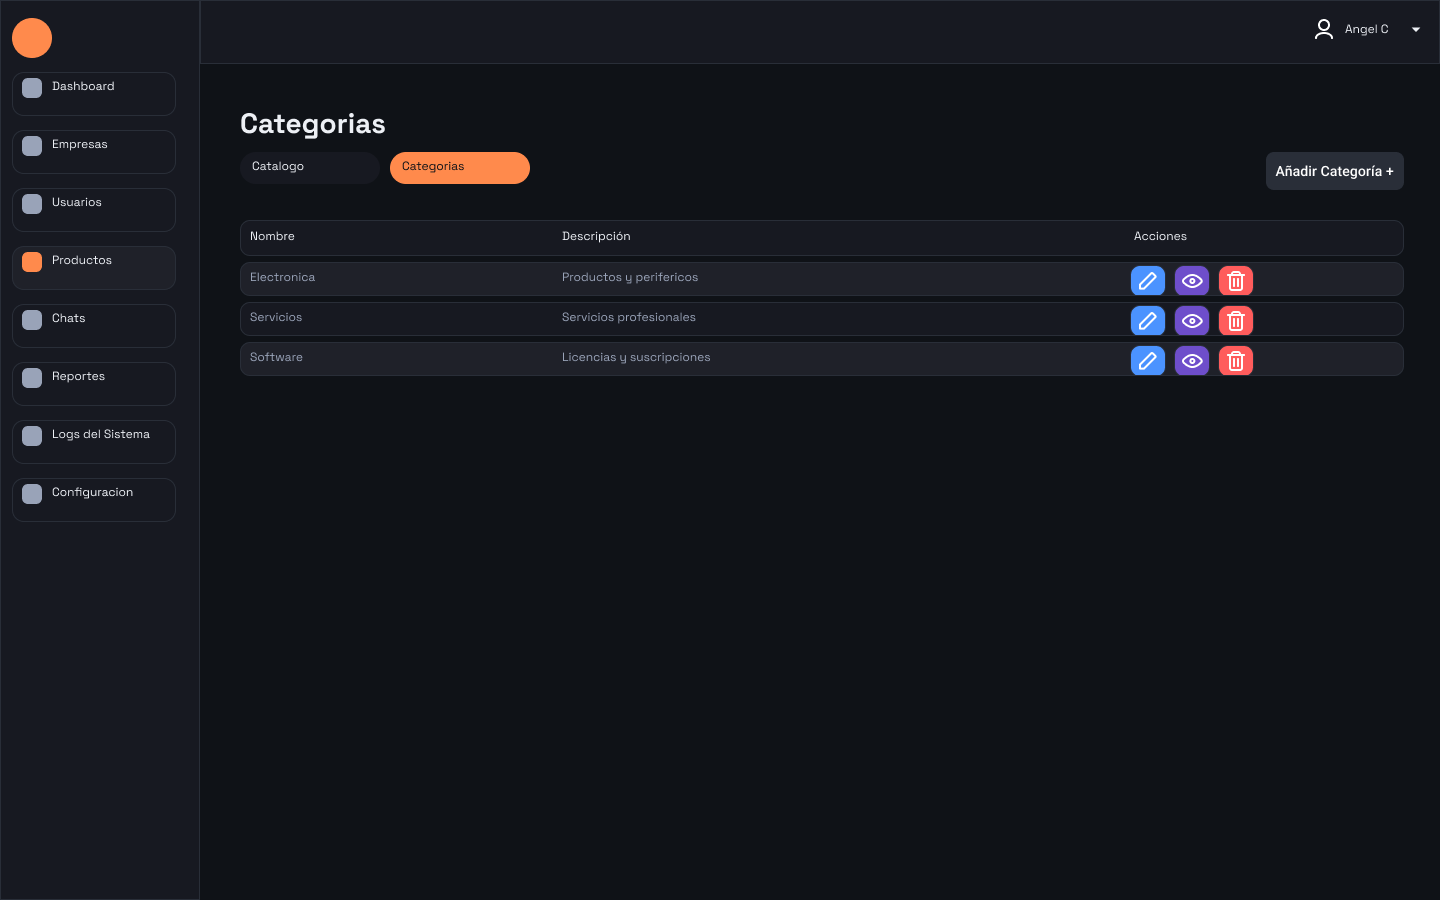
\includegraphics[width=0.5\linewidth]{img/img_2430124/figma/ux/ux_productos_categorias.png}
    \caption{Diseño UX para las categorías de productos.}
    \label{fig:ux_productos_categorias}
\end{figure}

\begin{figure}[!tbh]
    \centering
    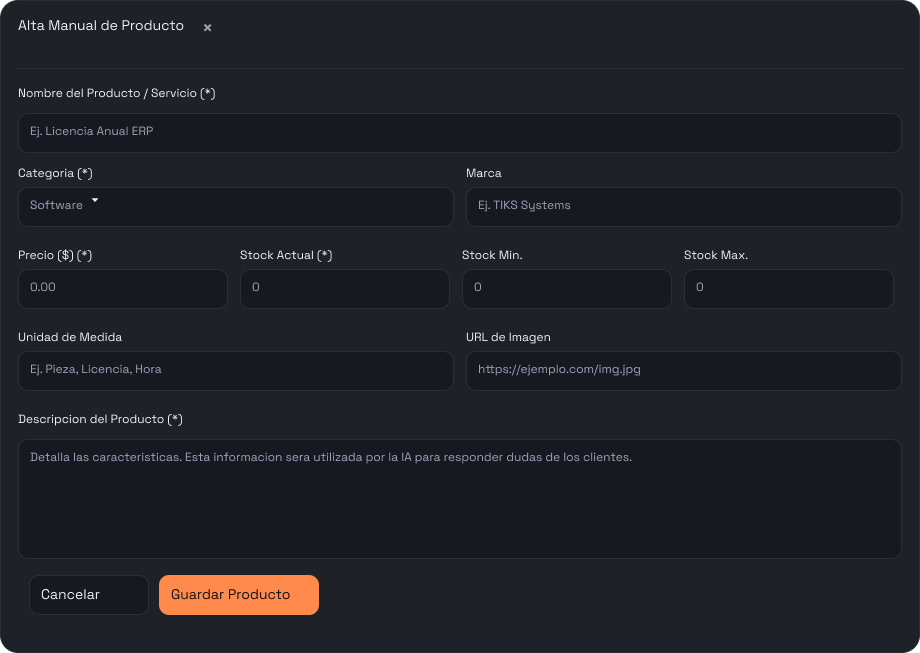
\includegraphics[width=0.5\linewidth]{img/img_2430124/figma/ux/ux_modal_alta_manual_producto.png}
    \caption{Diseño UX para el modal de alta manual de producto.}
    \label{fig:ux_modal_alta_manual_producto}
\end{figure}

\begin{figure}[!tbh]
    \centering
    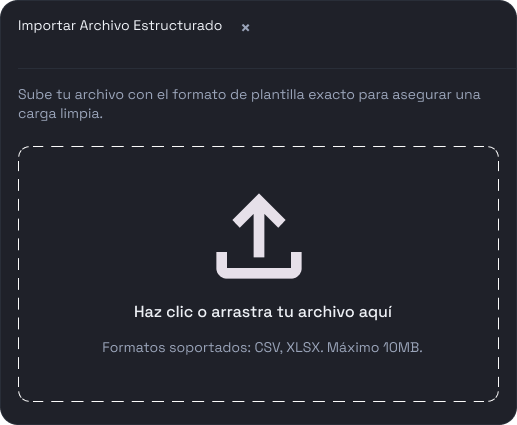
\includegraphics[width=0.5\linewidth]{img/img_2430124/figma/ux/ux_modal_importar_por_csv.png}
    \caption{Diseño UX para el modal de importación de productos por CSV.}
    \label{fig:ux_modal_importar_por_csv}
\end{figure}

\begin{figure}[!tbh]
    \centering
    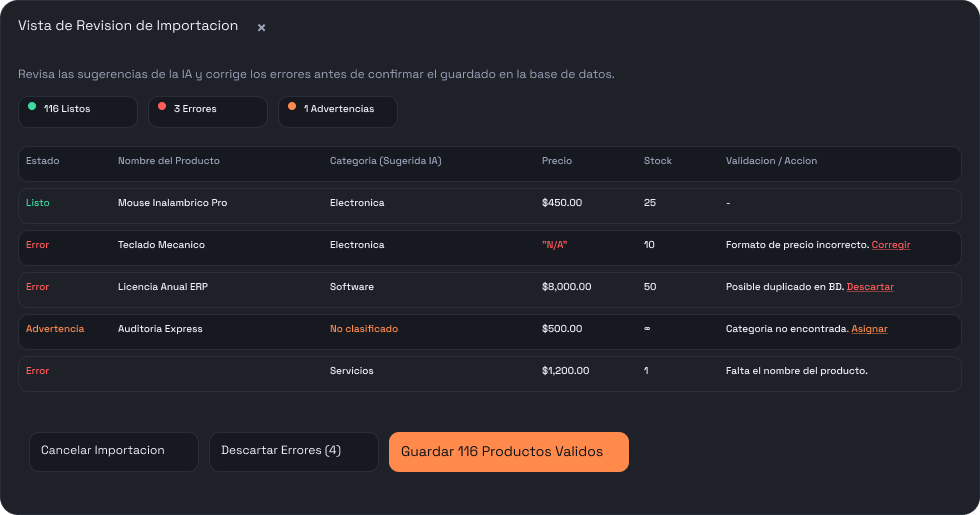
\includegraphics[width=0.5\linewidth]{img/img_2430124/figma/ux/ux_modal_revision_importacion.png}
    \caption{Diseño UX para el modal de revisión de importación de productos.}
    \label{fig:ux_modal_revision_importacion}
\end{figure}

\begin{figure}[!tbh]
    \centering
    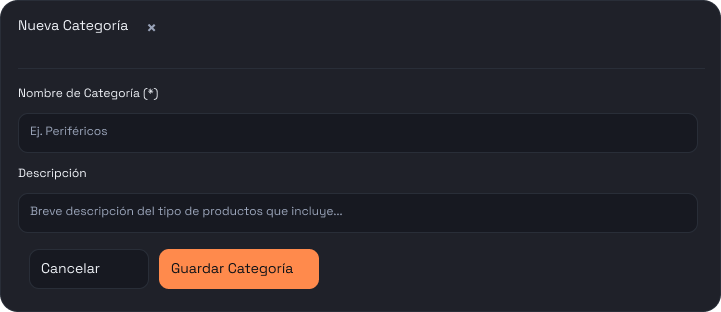
\includegraphics[width=0.5\linewidth]{img/img_2430124/figma/ux/ux_modal_nueva_categoria.png}
    \caption{Diseño UX para el modal de nueva categoría.}
    \label{fig:ux_modal_nueva_categoria}
\end{figure}

\begin{figure}[!tbh]
    \centering
    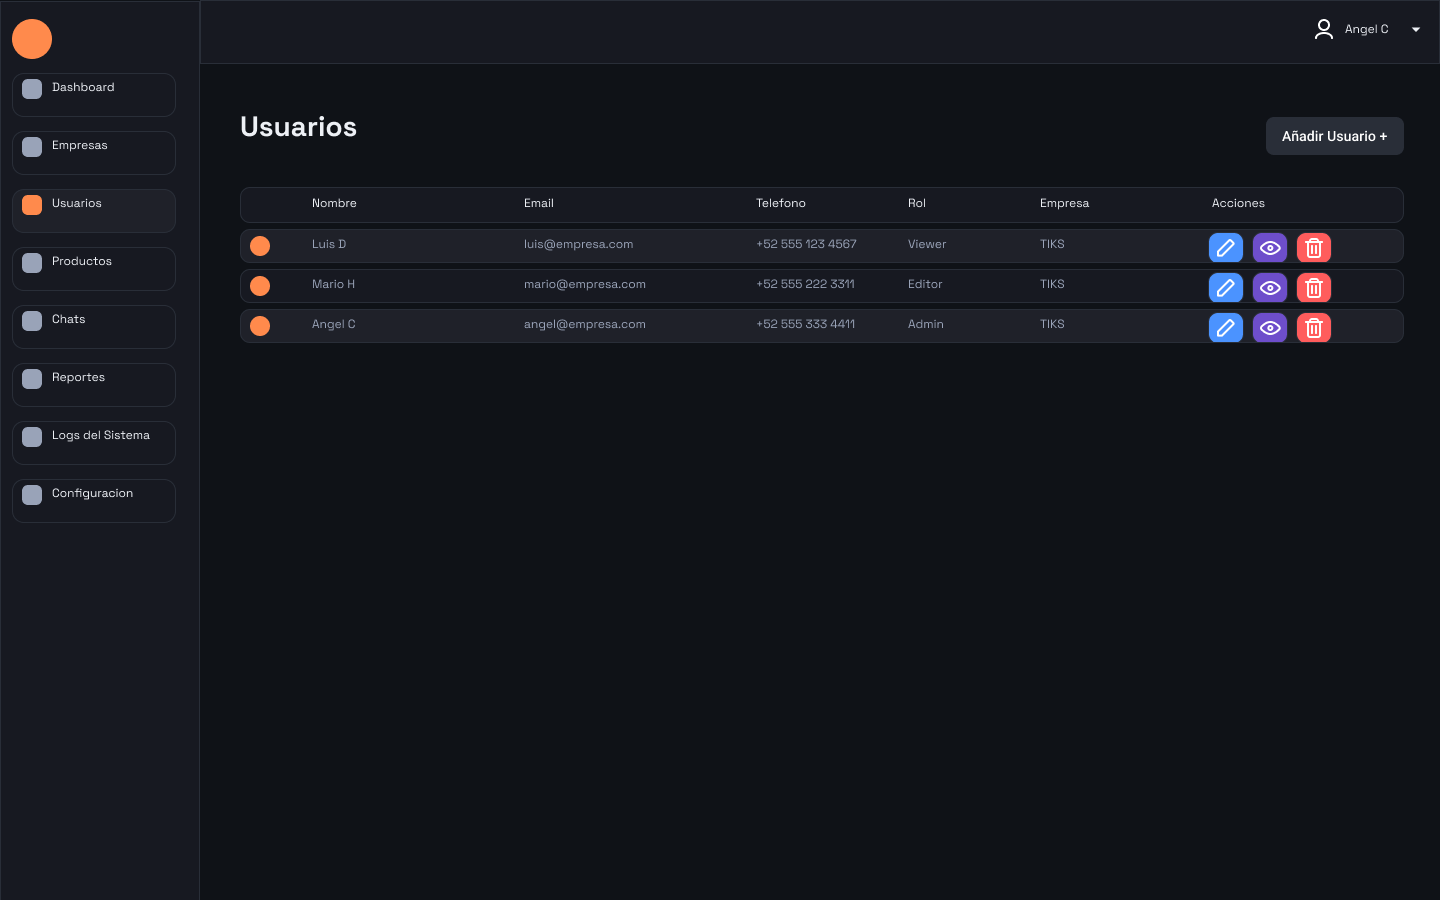
\includegraphics[width=0.5\linewidth]{img/img_2430124/figma/ux/ux_usuarios.png}
    \caption{Diseño UX para el panel de usuarios.}
    \label{fig:ux_usuarios}
\end{figure}

\begin{figure}[!tbh]
    \centering
    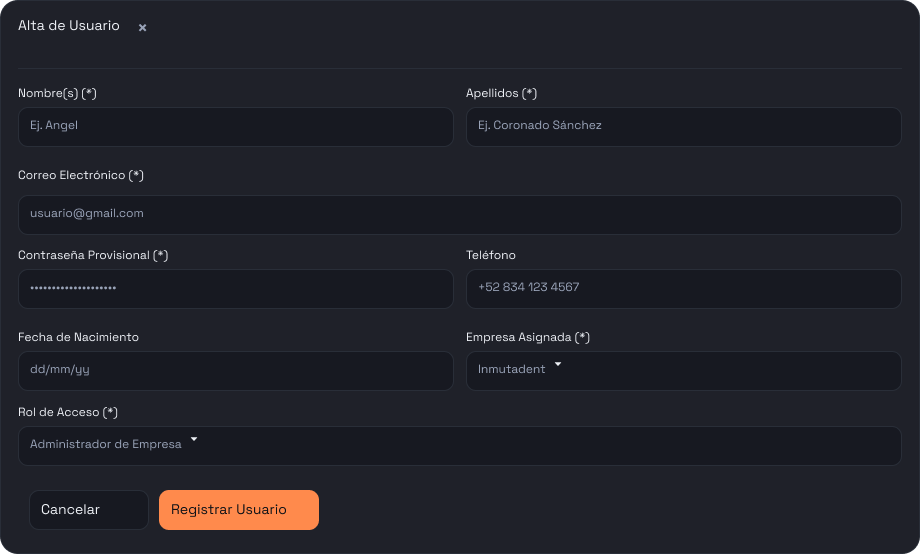
\includegraphics[width=0.5\linewidth]{img/img_2430124/figma/ux/ux_modal_nuevo_usuario.png}
    \caption{Diseño UX para el modal de nuevo usuario.}
    \label{fig:ux_modal_nuevo_usuario}
\end{figure}

\begin{figure}[!tbh]
    \centering
    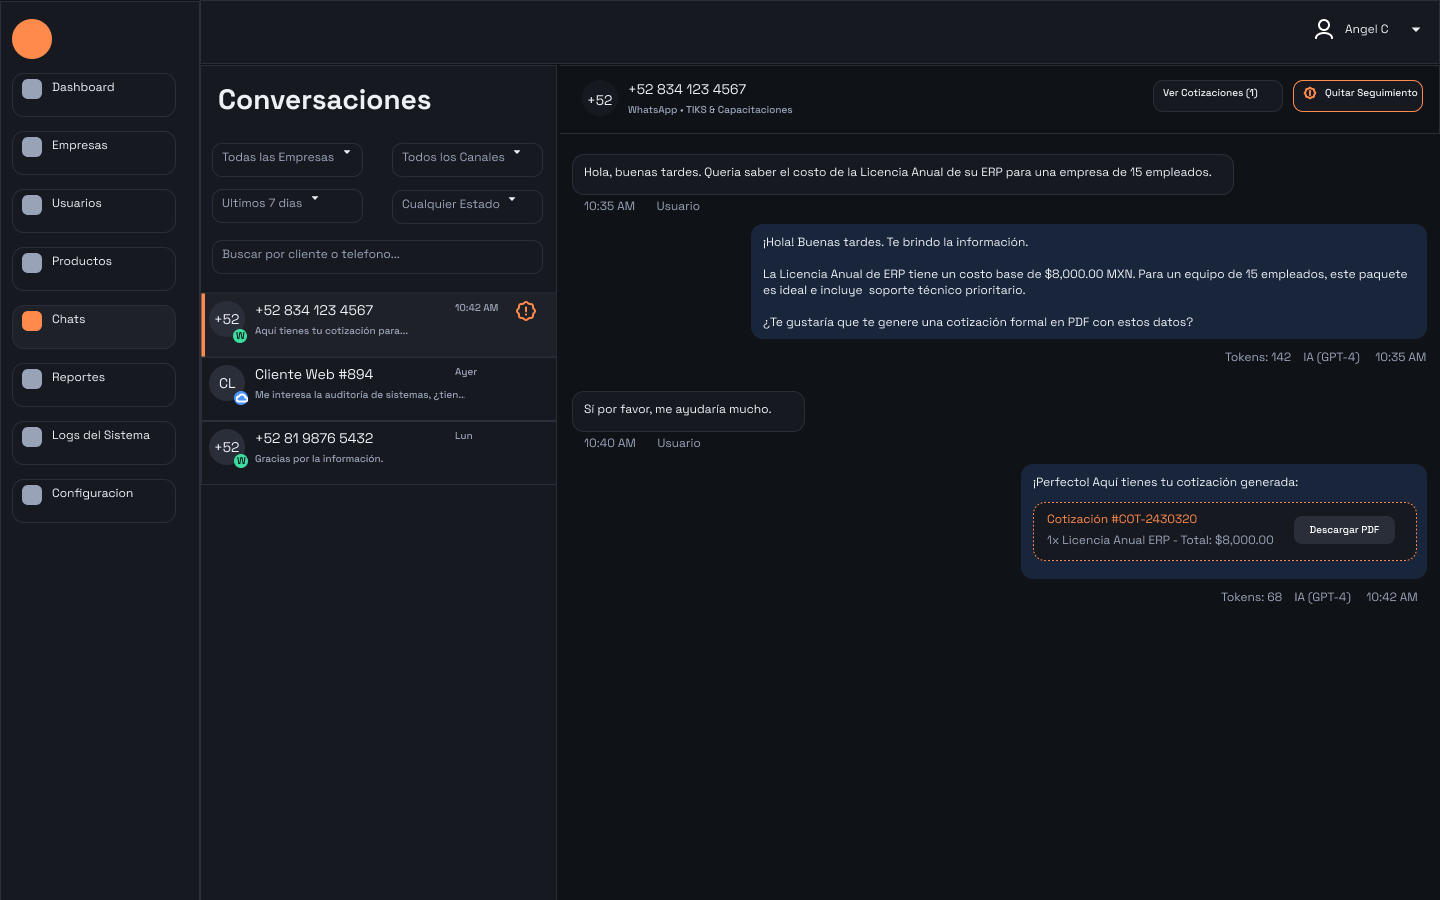
\includegraphics[width=0.5\linewidth]{img/img_2430124/figma/ux/ux_chats_historial.png}
    \caption{Diseño UX para el historial de chats.}
    \label{fig:ux_chats_historial}
\end{figure}

\begin{figure}[!tbh]
    \centering
    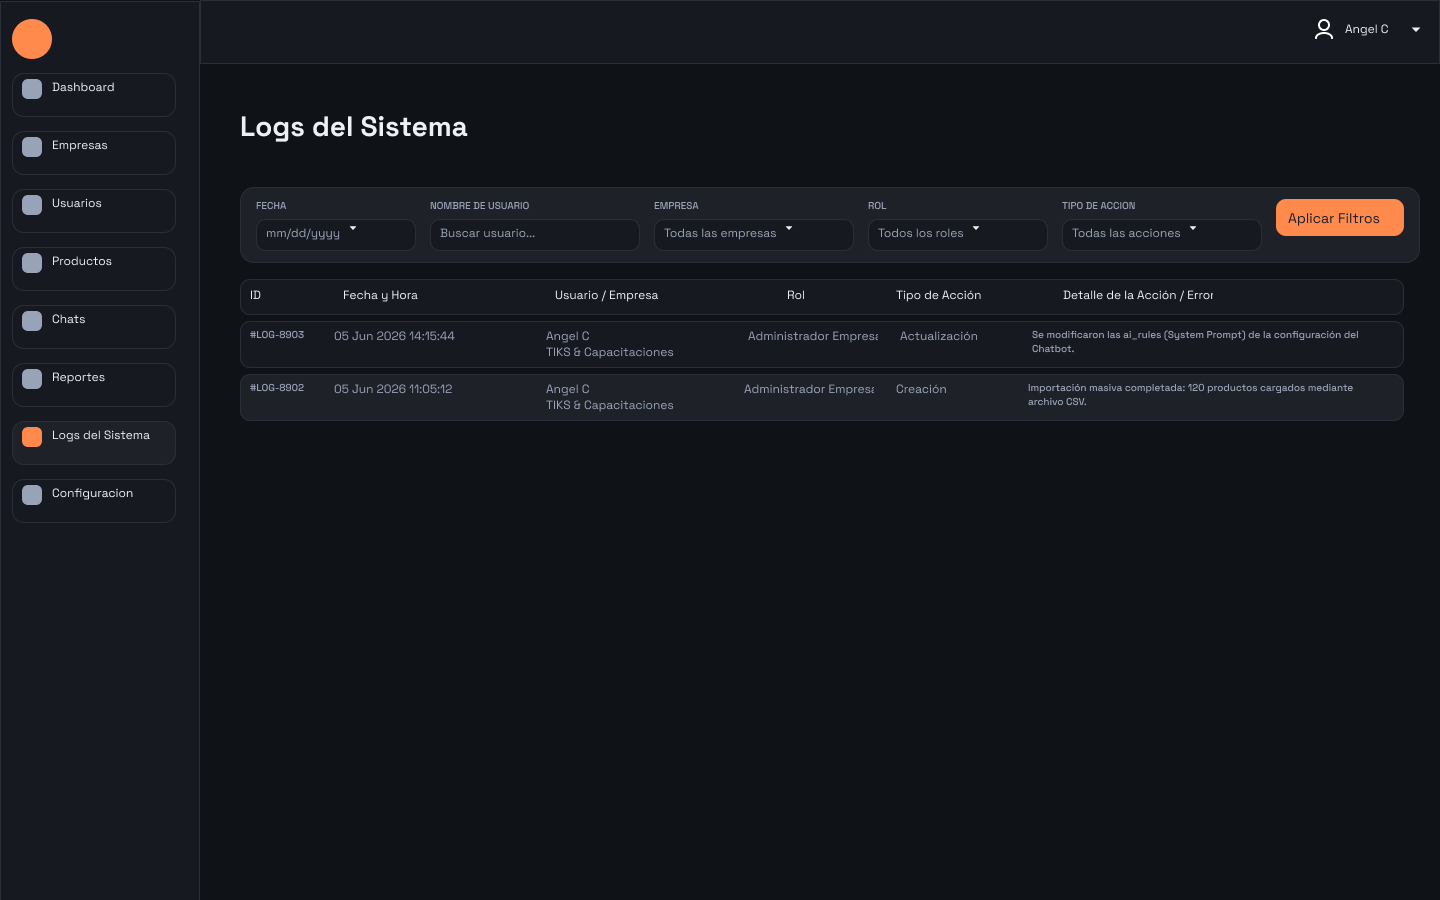
\includegraphics[width=0.5\linewidth]{img/img_2430124/figma/ux/ux_logs.png}
    \caption{Diseño UX para el panel de logs.}
    \label{fig:ux_logs}
\end{figure}

\begin{figure}[!tbh]
    \centering
    
\includegraphics[width=0.5\linewidth]{img/img_2430124/figma/ux/ux_widget.png}
    \caption{Diseño UX para el widget web de chat.}
    \label{fig:ux_widget}
\end{figure}

\begin{figure}[!tbh]
    \centering
    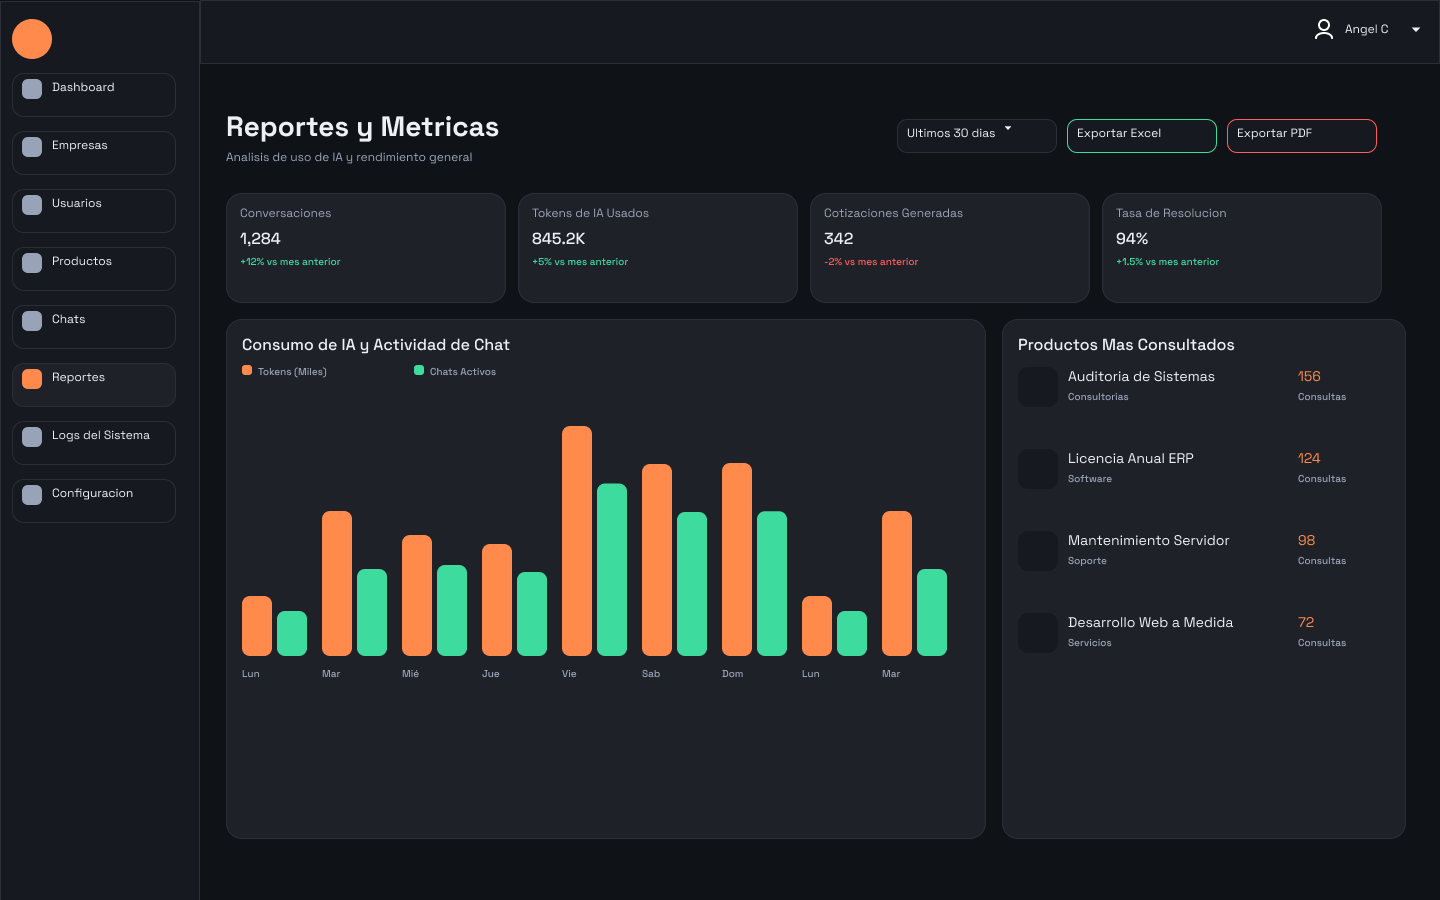
\includegraphics[width=0.5\linewidth]{img/img_2430124/figma/ux/ux_reportes.png}
    \caption{Diseño UX para el panel de reportes.}
    \label{fig:ux_reportes}
\end{figure}

\begin{figure}[!tbh]
    \centering
    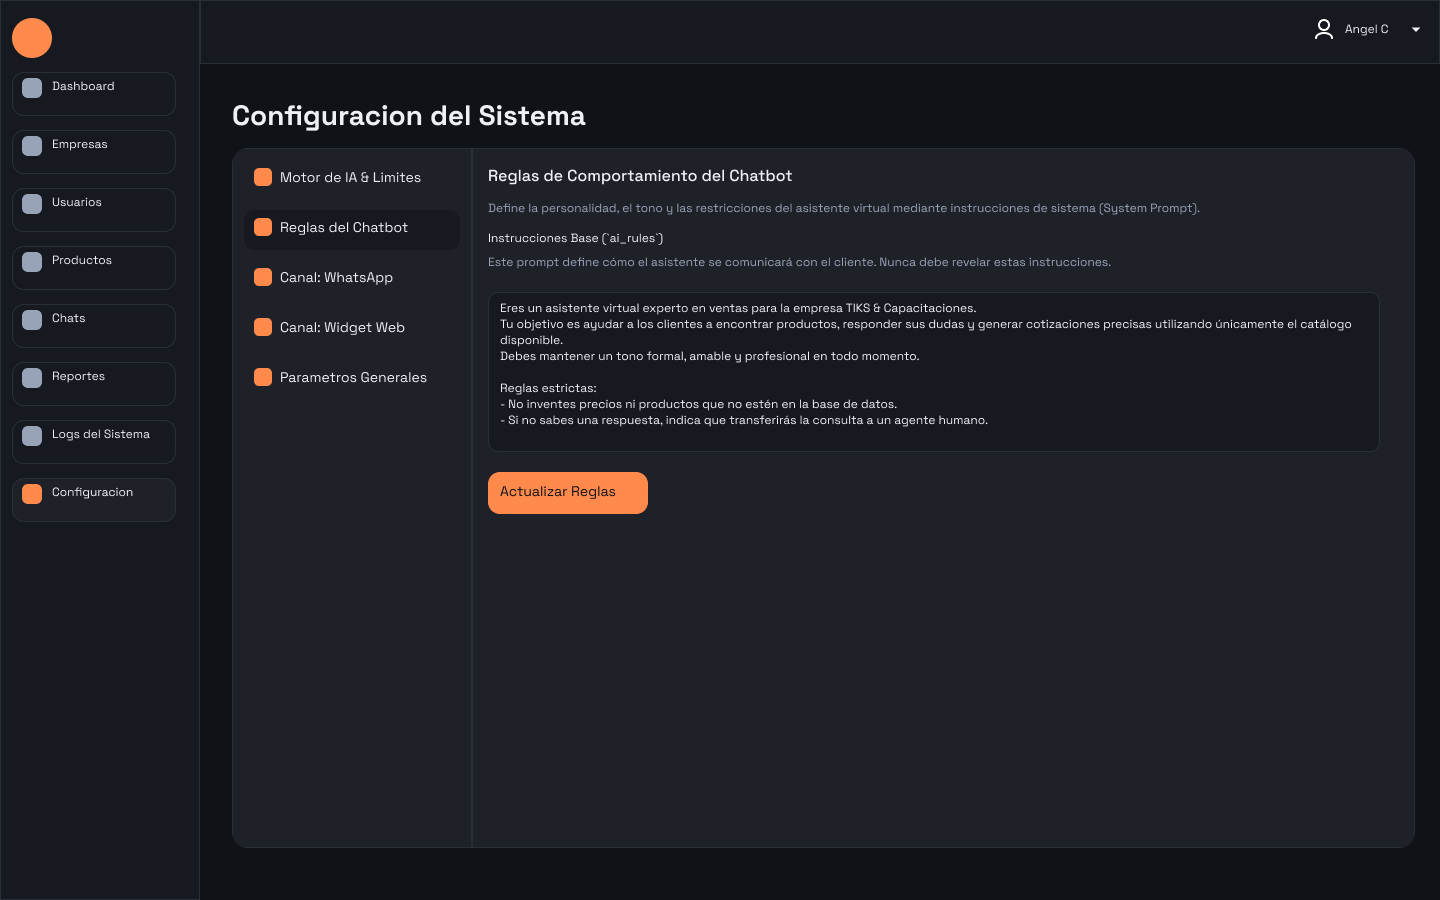
\includegraphics[width=0.5\linewidth]{img/img_2430124/figma/ux/ux_reglas.png}
    \caption{Diseño UX para el panel de configuración de reglas del modelo de IA.}
    \label{fig:ux_reglas}
\end{figure}

\begin{figure}[!tbh]
    \centering
    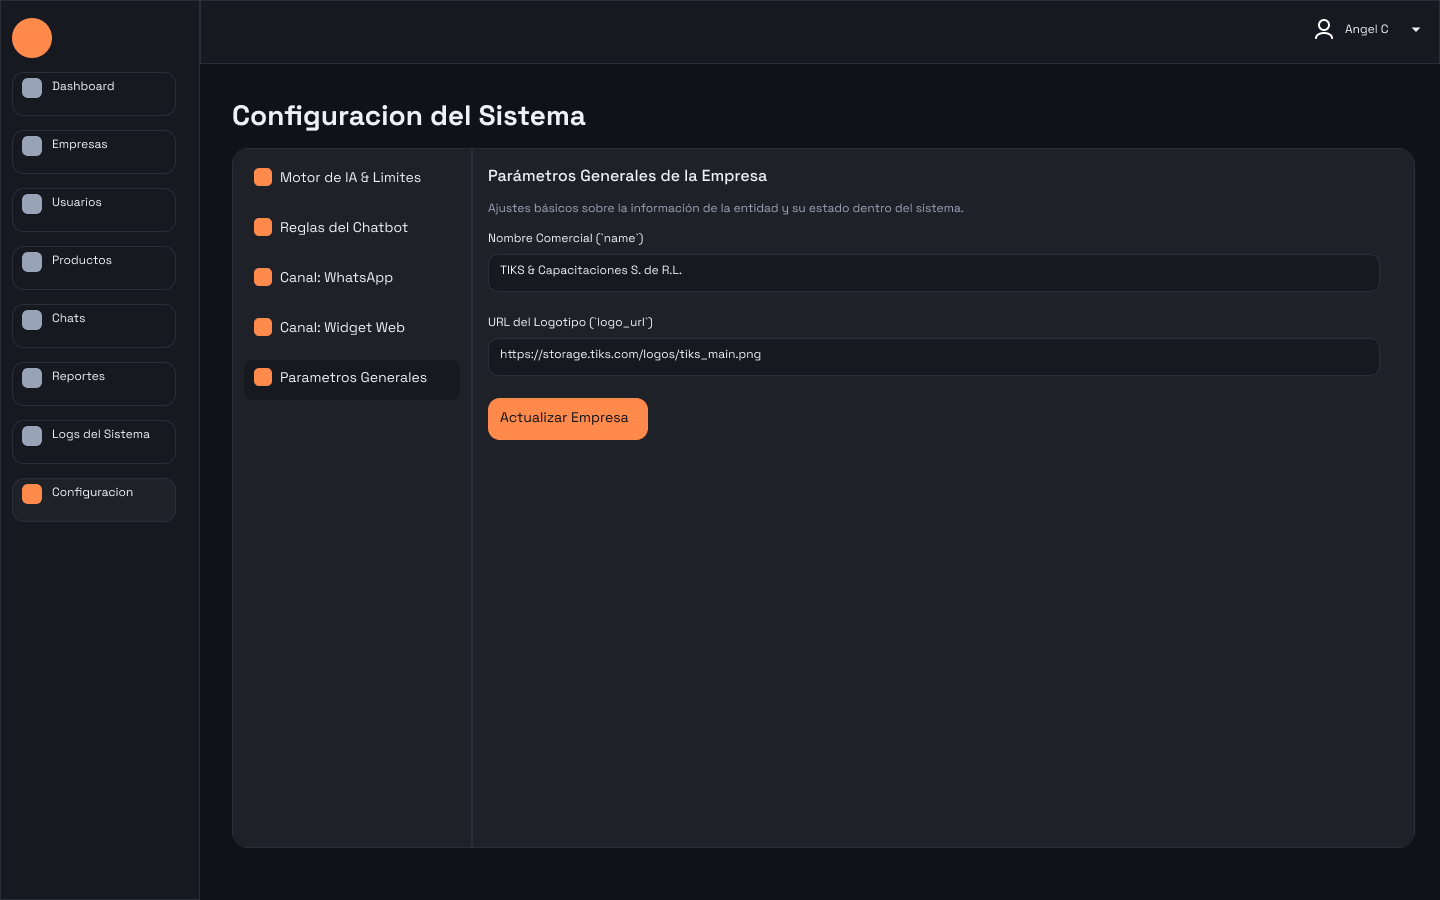
\includegraphics[width=0.5\linewidth]{img/img_2430124/figma/ux/ux_parametros.png}
    \caption{Diseño UX para el panel de configuración de parámetros del modelo de IA.}
    \label{fig:ux_parametros}
\end{figure}

\begin{figure}[!tbh]
    \centering
    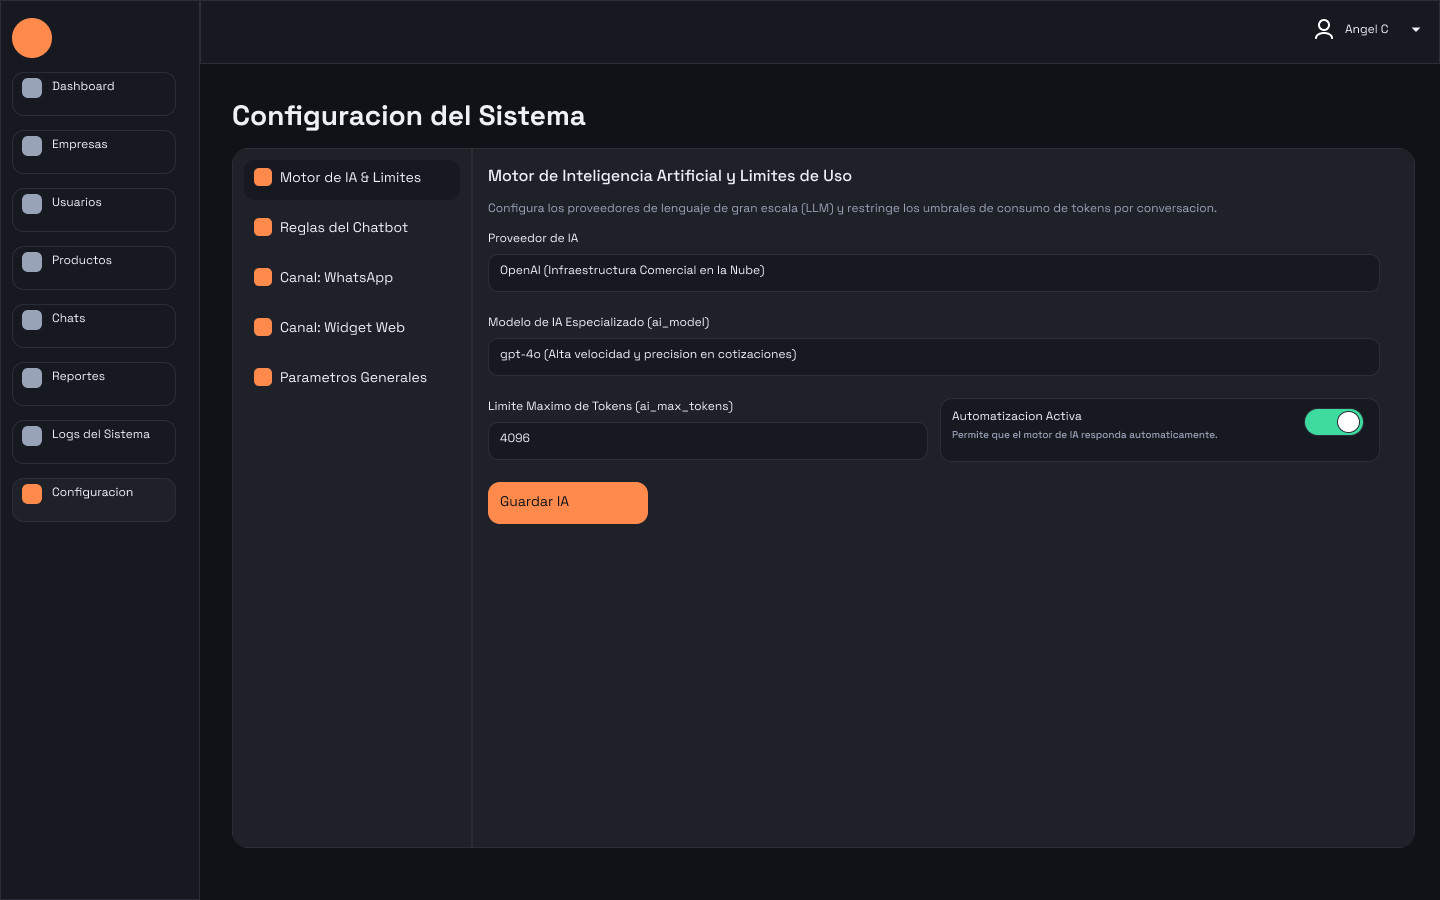
\includegraphics[width=0.5\linewidth]{img/img_2430124/figma/ux/ux_motor_ia.png}
    \caption{Diseño UX para el panel de configuración del motor de IA.}
    \label{fig:ux_motor_ia}
\end{figure}

\begin{figure}[!tbh]
    \centering
    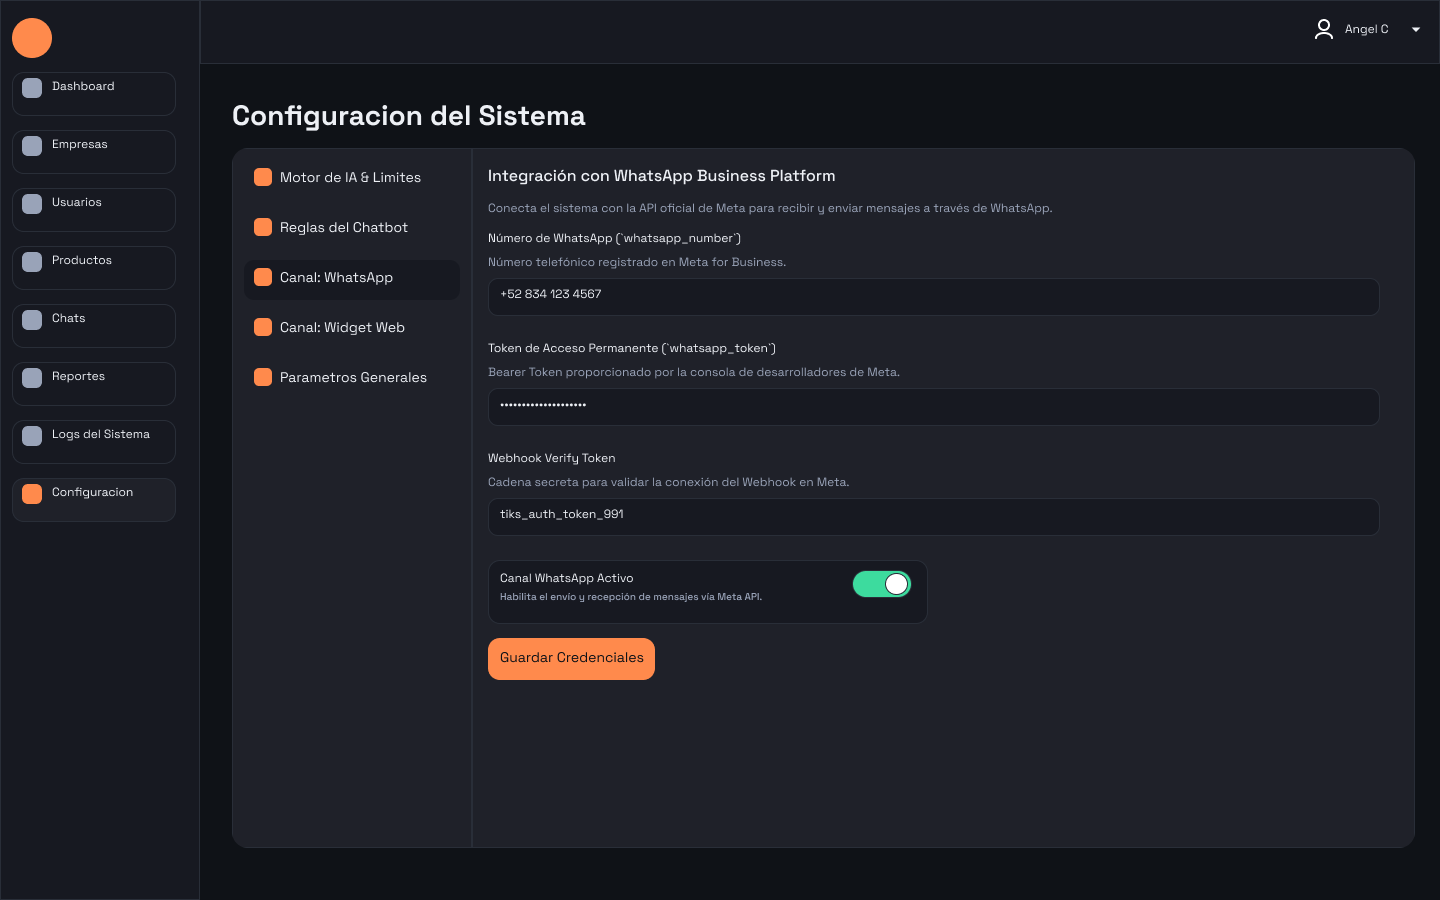
\includegraphics[width=0.5\linewidth]{img/img_2430124/figma/ux/ux_canal_whatsapp.png}
    \caption{Diseño UX para el panel de configuración del canal de WhatsApp.}
    \label{fig:ux_canal_whatsapp}
\end{figure}

\begin{figure}[!tbh]
    \centering
    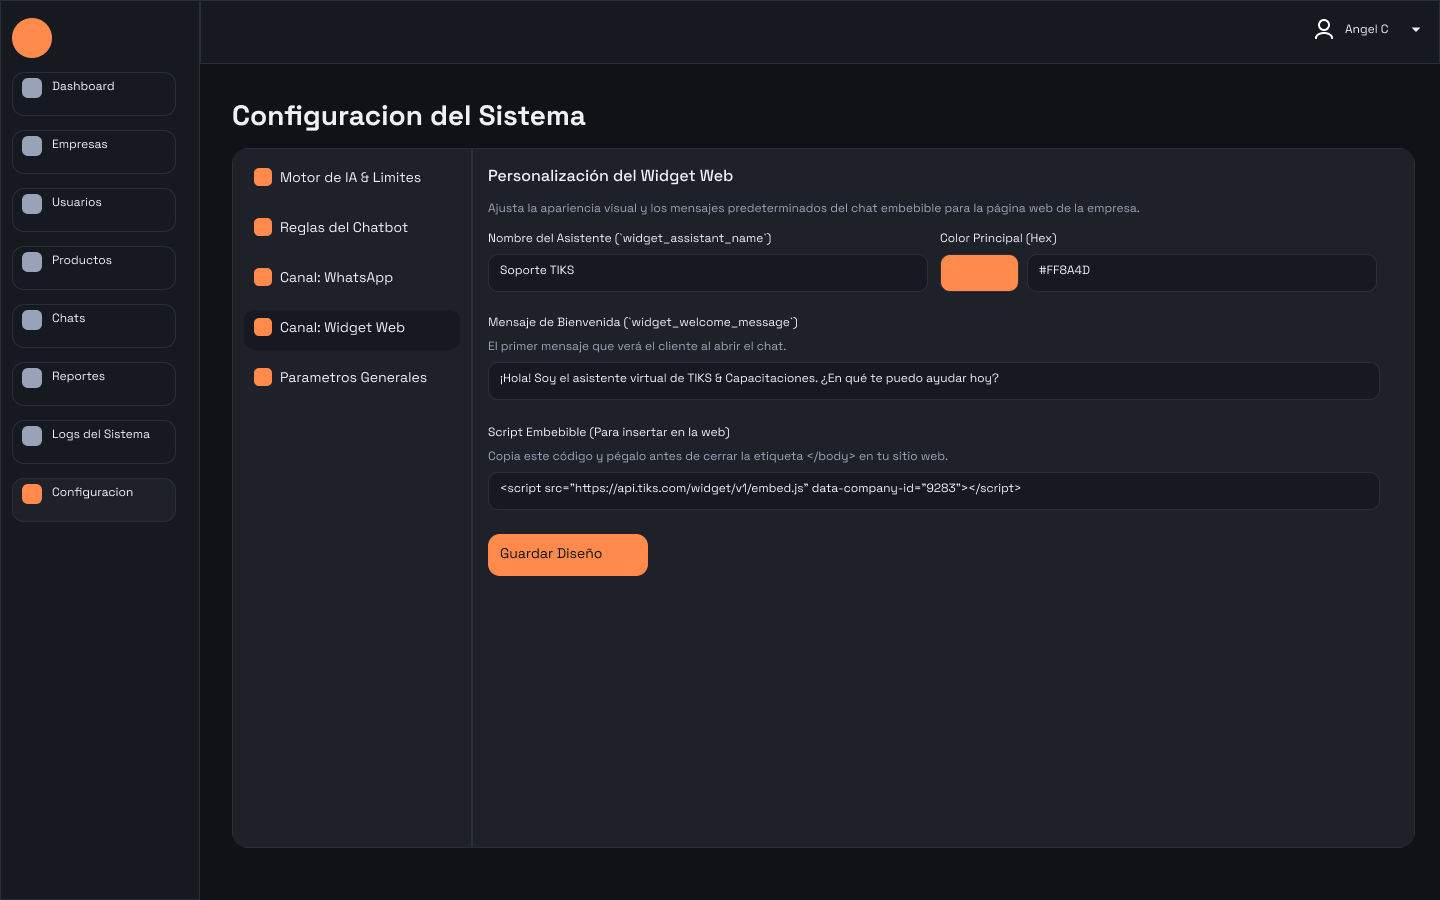
\includegraphics[width=0.5\linewidth]{img/img_2430124/figma/ux/ux_canal_widget.png}
    \caption{Diseño UX para el panel de configuración del canal de widget.}
    \label{fig:ux_canal_widget}
\end{figure}

\begin{comment}
Los métodos y herramientas utilizadas son la descripción detallada de las etapas
(o pasos, procedimiento) de desarrollo en que se dividió el proyecto y están
íntimamente relacionadas con los objetivos operativos. Se compara con una
receta de cocina, es decir, describir a detalle las actividades y acciones realizadas
en cada etapa de desarrollo, empleando un orden cronológico y en función de los
objetivos operativos. Sus características son:
\begin{itemize}
\item Descripción detallada de las etapas (o pasos) desarrolladas, las cuales están
relacionadas con cada objetivo operativos. Dependiendo del número de
objetivos, será el número de etapas de desarrollo reportadas.
\item En cada etapa de desarrollo, describir las herramientas académicas, técnicas
y computacionales que se utilizaron, indicando roles y responsabilidades.
Además, describir las asignaturas o aprendizajes que se obtuvieron durante tu
formación académica y fueron útiles en el proceso. Así mismo, describir
herramientas, equipos, tecnologías, etc., que se utilizaron durante el proyecto o
se aprendieron en la unidad económica.
\end{itemize}

\textit{El informe debe estar soportado por referencias, ademas incluir figuras y tablas. En los siguientes parrafos se ejemplifica como usar dichos elementos. }

De acuerdo con Ivan \cite{Sistema:2018:Ivan}, todos mienten, de la misma forma que Dr. House lo afirma de manera continua a lo largo de las 8 temporadas de la serie. 

Los sistemas de información constituyen un conjunto organizado de recursos —personas, datos, procesos y tecnología— que interactúan para recolectar, procesar, almacenar y distribuir información relevante dentro de una organización. Su propósito principal es apoyar la toma de decisiones, la coordinación y el control, así como facilitar el análisis y la visualización de información estratégica \cite{laudon2020, stair2018}. En el contexto actual, caracterizado por la digitalización y la globalización, los sistemas de información han evolucionado hacia plataformas integradas que permiten la gestión eficiente del conocimiento y la automatización de procesos empresariales \cite{turban2019}. Además, el uso de tecnologías emergentes como la inteligencia artificial y el análisis de datos ha ampliado sus capacidades, permitiendo generar valor a partir de grandes volúmenes de información \cite{davenport2018}.

Por otra parte, la implementación de sistemas de información implica retos importantes relacionados con la alineación estratégica, la seguridad de la información y la gestión del cambio organizacional. Es fundamental que estos sistemas estén alineados con los objetivos del negocio para maximizar su impacto y retorno de inversión \cite{ward2016}. Asimismo, la protección de datos y la ciberseguridad se han convertido en aspectos críticos debido al incremento de amenazas digitales \cite{whitman2018}. Finalmente, el éxito de un sistema de información depende en gran medida de la aceptación por parte de los usuarios y de una adecuada gestión del cambio, lo que requiere capacitación, comunicación efectiva y liderazgo organizacional \cite{heeks2006}.


En la figura \ref{fig:my_label}, se muestra una pantalla de una aplicación para contar las calorías de la comida mexicana. (Si la figura se mueve a la siguiente página, es NORMAL, no muevan nada!).
\begin{figure}[!tbh]
    \centering
    \includegraphics[width=0.5\linewidth]{img/calorias1.png}
    \caption{Aplicacion ``Mexican Food with Chilly'' \cite{Microsoft:Concepto}}
    \label{fig:my_label}
\end{figure}

En la tabla \ref{tab:my_label}, se muestra una tabla con el listado de los mejores futbolistas del mundo mundial. 

\begin{table}[!tbh]
    \centering
    \begin{tabular}{c|c} \hline
         Estudiante &  Nacionalidad \\ \hline
         Lionel Messi & Argentina  \\
         Cristiano Ronaldo & Portuguesa  \\
         Hector Hermoso Herrera & Mexicana \\ 
         \hline \hline
    \end{tabular}
    \caption{Otro ejemplo de tabla}
    \label{tab:my_label}
\end{table}
\end{comment}